\documentclass[12pt,a4paper]{article}

% ============================================================================
% Packages
% ============================================================================
\usepackage[margin=1in]{geometry}
\usepackage{graphicx}
\usepackage{xcolor}
\usepackage{hyperref}
\usepackage{listings}
\usepackage{booktabs}
\usepackage{longtable}
\usepackage{tabularx}
\usepackage{float}
\usepackage{amsmath}
\usepackage{fancyhdr}
\usepackage{caption}
\usepackage{subcaption}
\usepackage{tikz}
\usetikzlibrary{shapes.geometric, arrows.meta, positioning, fit, calc}
\usepackage[T1]{fontenc}
\usepackage{lmodern}
\usepackage{microtype}
\usepackage{parskip}

% ============================================================================
% Theme & Colors
% ============================================================================
\definecolor{codeblue}{HTML}{0077B6}
\definecolor{codegray}{HTML}{5A5A5A}
\definecolor{codegreen}{HTML}{2D6A4F}
\definecolor{codebg}{HTML}{F8F9FA}
\definecolor{accentcyan}{HTML}{00D4FF}
\definecolor{accentred}{HTML}{FF4E42}
\definecolor{accentorange}{HTML}{FF7B39}
\definecolor{titleblue}{HTML}{1B263B}

\hypersetup{
  colorlinks=true,
  linkcolor=codeblue,
  urlcolor=codeblue,
  citecolor=codeblue,
}

% ============================================================================
% Code Listings
% ============================================================================
\lstdefinestyle{codestyle}{
  backgroundcolor=\color{codebg},
  basicstyle=\ttfamily\small,
  breakatwhitespace=false,
  breaklines=true,
  captionpos=b,
  commentstyle=\color{codegreen},
  keywordstyle=\color{codeblue}\bfseries,
  stringstyle=\color{accentorange},
  numberstyle=\tiny\color{codegray},
  numbers=left,
  numbersep=8pt,
  frame=single,
  rulecolor=\color{codegray!30},
  tabsize=2,
  showstringspaces=false,
  xleftmargin=1.5em,
  framexleftmargin=1em,
}
\lstset{style=codestyle}

% ============================================================================
% Header / Footer
% ============================================================================
\pagestyle{fancy}
\fancyhf{}
\fancyhead[L]{\small\textsc{WhiteChristmas}}
\fancyhead[R]{\small\textsc{Real-Time Crime Analytics Platform}}
\fancyfoot[C]{\thepage}
\renewcommand{\headrulewidth}{0.4pt}

% ============================================================================
% Title
% ============================================================================
\title{
  \vspace{-1cm}
  {\Huge\bfseries\color{titleblue} WhiteChristmas}\\[0.3cm]
  {\Large Real-Time Crime Analytics \& Intelligence Platform}\\[0.3cm]
  {\large A Polyglot Streaming Pipeline for Chicago Public Safety Data}\\[0.5cm]
  \rule{\textwidth}{0.5pt}
}
\author{
  \textbf{Arqam Zia}\\
  \texttt{i221170@nu.edu.pk}
  \and
  \textbf{Danish Haroon}\\
  \texttt{i220955@nu.edu.pk}
}
\date{May 2026}

% ============================================================================
% Document
% ============================================================================
\begin{document}
\maketitle
\thispagestyle{empty}

\vfill
\begin{abstract}
\noindent
WhiteChristmas is a polyglot, real-time crime analytics platform that ingests, processes, and visualizes Chicago public safety data across five datasets: crimes (2001--present), arrests, violence reduction (homicides and non-fatal shootings), sex offender registrations, and police station locations. The system implements a hybrid Lambda/Kappa architecture using Rust for high-throughput data ingestion, Apache Kafka (KRaft mode) as the messaging backbone with Confluent Avro serialization, Apache Spark Structured Streaming (Scala) for windowed aggregations and statistical anomaly detection, Go for real-time WebSocket delivery and REST API serving, PostgreSQL and MongoDB for dual-model persistence, and a Next.js dashboard with ECharts and Leaflet for interactive visualization. Observability is provided through Prometheus metrics collection and Grafana dashboards. The entire platform is orchestrated via Docker Compose and processes approximately 199,000+ events across the pipeline with sub-second alert latency.
\end{abstract}
\vfill

\newpage
\tableofcontents
\newpage

% ============================================================================
% 1. INTRODUCTION
% ============================================================================
\section{Introduction}

\subsection{Motivation}

Urban crime analytics is a domain where timely data processing can directly impact public safety outcomes. The City of Chicago publishes extensive public safety datasets through its open data portal, spanning over two decades of crime records, arrest data, violence reduction statistics, sex offender registrations, and police infrastructure data. These datasets, totaling over 2.5~GB of raw CSV data, present both an opportunity and a challenge: the opportunity to derive real-time intelligence from historical patterns, and the challenge of building a system that can ingest, normalize, process, and present this data with minimal latency.

WhiteChristmas addresses this challenge by constructing a full-stack streaming analytics platform that treats these static datasets as continuous event streams, enabling real-time anomaly detection, statistical analysis, and interactive visualization.

\subsection{Project Scope}

The platform encompasses:
\begin{itemize}
  \item Real-time streaming ingestion of five Chicago public safety CSV datasets
  \item Unified event normalization via Apache Avro with Schema Registry
  \item Dual-path processing: Spark Structured Streaming (real-time) and Spark Batch (historical)
  \item Statistical anomaly detection using z-score analysis and volume thresholds
  \item WebSocket-based real-time event delivery to browser clients
  \item Interactive dashboard with 10+ data visualizations, heatmaps, and historical replay
  \item Full observability stack with Prometheus and Grafana
  \item Containerized deployment via Docker Compose (12 services)
\end{itemize}

\subsection{Technology Selection Rationale}

The polyglot architecture was chosen deliberately to leverage each language's strengths:

\begin{table}[H]
\centering
\caption{Language selection rationale}
\begin{tabularx}{\textwidth}{l l X}
\toprule
\textbf{Component} & \textbf{Language} & \textbf{Rationale} \\
\midrule
Data Ingestion & Rust & Zero-cost abstractions, memory safety without GC, high-throughput async I/O via Tokio \\
Stream Processing & Scala & Native Spark API, functional paradigm for data transformations, JVM ecosystem \\
API \& WebSocket & Go & Lightweight goroutines for concurrent WebSocket connections, fast compilation \\
Frontend & TypeScript & React/Next.js ecosystem, type safety, ECharts integration \\
\bottomrule
\end{tabularx}
\end{table}

% ============================================================================
% 2. SYSTEM ARCHITECTURE
% ============================================================================
\section{System Architecture}

\subsection{Architectural Overview}

WhiteChristmas implements a \textbf{hybrid Lambda/Kappa architecture}. The Kappa path handles real-time event processing through Spark Structured Streaming, while the Lambda batch path runs periodic Spark batch jobs for historical aggregations that are too expensive to compute in real-time.

\begin{figure}[H]
\centering
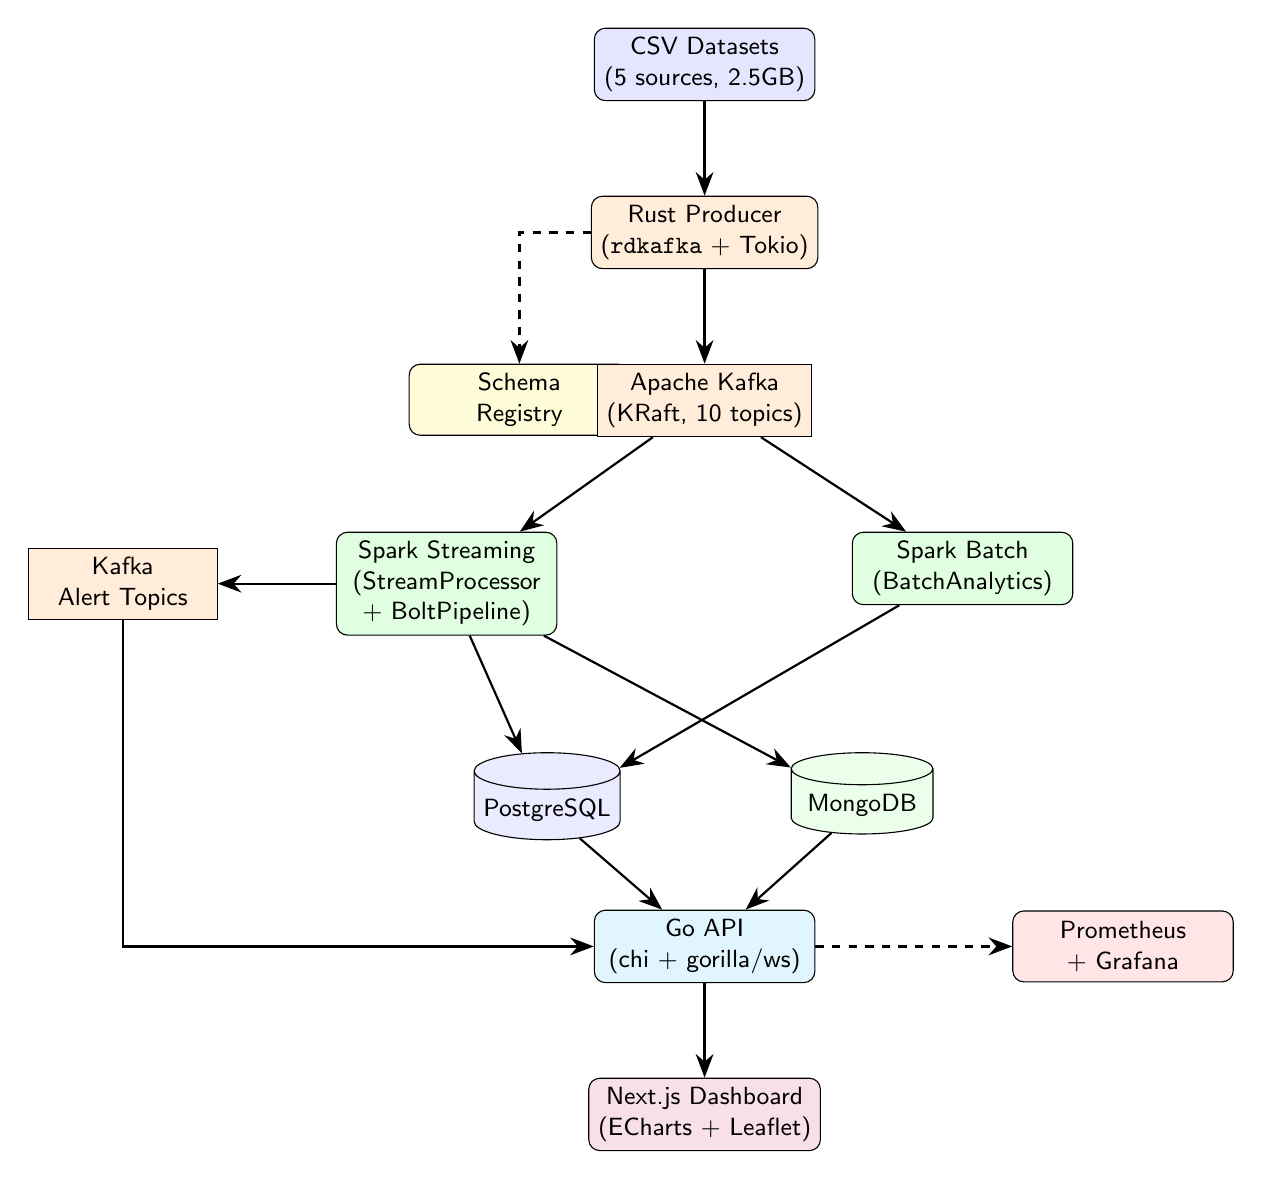
\begin{tikzpicture}[
  node distance=1.2cm and 2cm,
  block/.style={rectangle, draw, rounded corners, minimum width=2.8cm, minimum height=0.9cm, align=center, font=\small\sffamily},
  store/.style={cylinder, draw, shape border rotate=90, minimum width=1.8cm, minimum height=0.9cm, aspect=0.25, align=center, font=\small\sffamily},
  topic/.style={rectangle, draw, fill=orange!15, minimum width=2.4cm, minimum height=0.7cm, align=center, font=\small\sffamily},
  arr/.style={-{Stealth[length=3mm]}, thick},
]

% Row 1: Data Sources
\node[block, fill=blue!10] (csv) {CSV Datasets\\(5 sources, 2.5GB)};

% Row 2: Ingestion
\node[block, fill=orange!15, below=of csv] (rust) {Rust Producer\\(\texttt{rdkafka} + Tokio)};

% Row 3: Schema + Kafka
\node[block, fill=yellow!15, below left=1.2cm and -0.5cm of rust] (sr) {Schema\\Registry};
\node[topic, below=of rust] (kafka) {Apache Kafka\\(KRaft, 10 topics)};

% Row 4: Processing
\node[block, fill=green!12, below left=1.2cm and 0.5cm of kafka] (stream) {Spark Streaming\\(StreamProcessor\\+ BoltPipeline)};
\node[block, fill=green!12, below right=1.2cm and 0.5cm of kafka] (batch) {Spark Batch\\(BatchAnalytics)};

% Row 5: Storage
\node[store, fill=blue!8, below=4cm of kafka, xshift=-2cm] (pg) {PostgreSQL};
\node[store, fill=green!8, below=4cm of kafka, xshift=2cm] (mongo) {MongoDB};

% Row 5b: Alert topics
\node[topic, left=1.5cm of stream] (alerts) {Kafka\\Alert Topics};

% Row 6: API
\node[block, fill=cyan!12, below=6cm of kafka] (api) {Go API\\(chi + gorilla/ws)};

% Row 7: Frontend
\node[block, fill=purple!12, below=of api] (fe) {Next.js Dashboard\\(ECharts + Leaflet)};

% Row 6b: Observability
\node[block, fill=red!10, right=2.5cm of api] (prom) {Prometheus\\+ Grafana};

% Arrows
\draw[arr] (csv) -- (rust);
\draw[arr] (rust) -- (kafka);
\draw[arr, dashed] (rust) -| (sr);
\draw[arr] (kafka) -- (stream);
\draw[arr] (kafka) -- (batch);
\draw[arr] (stream) -- (pg);
\draw[arr] (stream) -- (mongo);
\draw[arr] (stream) -- (alerts);
\draw[arr] (batch) -- (pg);
\draw[arr] (alerts) |- (api);
\draw[arr] (pg) -- (api);
\draw[arr] (mongo) -- (api);
\draw[arr] (api) -- (fe);
\draw[arr, dashed] (api) -- (prom);

\end{tikzpicture}
\caption{High-level system architecture diagram}
\label{fig:arch}
\end{figure}

\subsection{Data Flow}

The end-to-end data flow proceeds through five stages:

\begin{enumerate}
  \item \textbf{Ingestion:} The Rust producer reads CSV files, normalizes rows into a unified Avro schema, and publishes to per-dataset Kafka topics at a configurable rate (default: 10 events/sec/dataset).
  \item \textbf{Streaming Processing:} Spark Structured Streaming consumes from \texttt{raw-events-*} topics, applies windowed aggregations, z-score anomaly detection, and volume threshold monitoring, then writes enriched events to PostgreSQL and alerts to MongoDB and Kafka alert topics.
  \item \textbf{Batch Processing:} On-demand Spark batch jobs read the raw CSV files directly to compute historical aggregations (crime trends, arrest rates, hotspot clustering, cross-dataset correlations) and write results to PostgreSQL.
  \item \textbf{Serving:} The Go API consumes alert topics from Kafka and broadcasts to WebSocket clients in real-time, while also serving REST endpoints backed by PostgreSQL and MongoDB queries.
  \item \textbf{Visualization:} The Next.js dashboard connects via WebSocket for live events and polls REST endpoints at varying intervals (2s--5min) for analytics data.
\end{enumerate}

\begin{figure}[H]
\centering
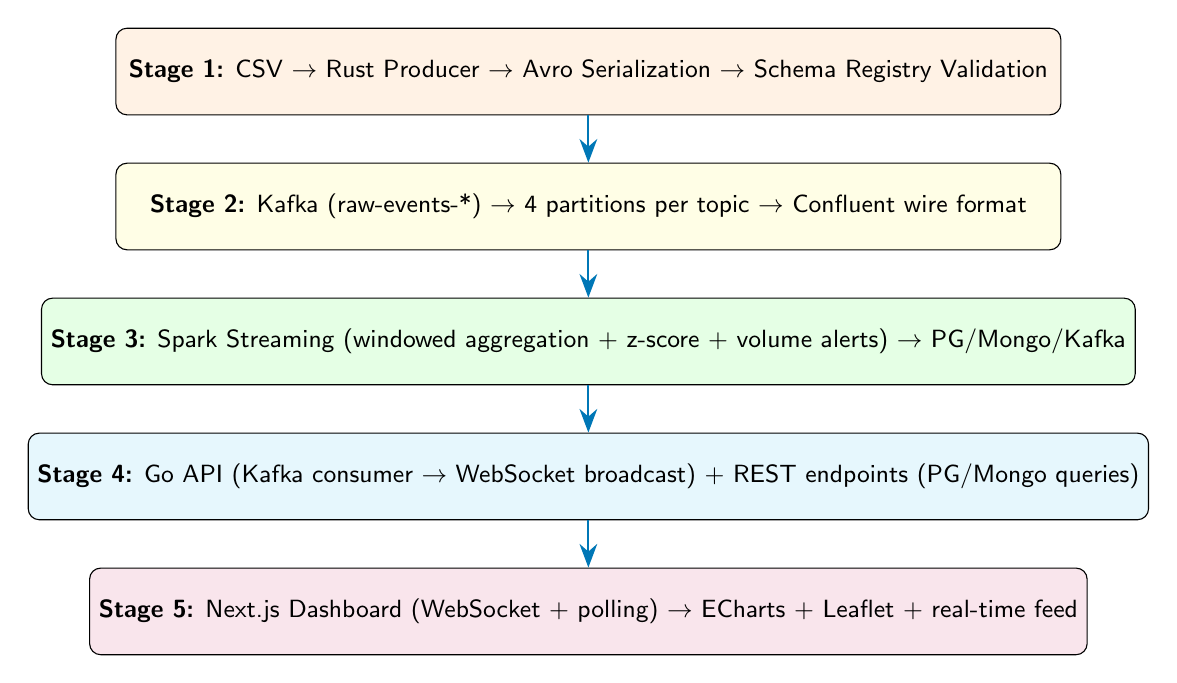
\begin{tikzpicture}[
  node distance=0.6cm,
  stage/.style={rectangle, draw, rounded corners, minimum width=12cm, minimum height=1.1cm, align=center, font=\small\sffamily},
  arr/.style={-{Stealth[length=3mm]}, thick, color=codeblue},
]
\node[stage, fill=orange!10] (s1) {\textbf{Stage 1:} CSV $\rightarrow$ Rust Producer $\rightarrow$ Avro Serialization $\rightarrow$ Schema Registry Validation};
\node[stage, fill=yellow!10, below=of s1] (s2) {\textbf{Stage 2:} Kafka (raw-events-*) $\rightarrow$ 4 partitions per topic $\rightarrow$ Confluent wire format};
\node[stage, fill=green!10, below=of s2] (s3) {\textbf{Stage 3:} Spark Streaming (windowed aggregation + z-score + volume alerts) $\rightarrow$ PG/Mongo/Kafka};
\node[stage, fill=cyan!10, below=of s3] (s4) {\textbf{Stage 4:} Go API (Kafka consumer $\rightarrow$ WebSocket broadcast) + REST endpoints (PG/Mongo queries)};
\node[stage, fill=purple!10, below=of s4] (s5) {\textbf{Stage 5:} Next.js Dashboard (WebSocket + polling) $\rightarrow$ ECharts + Leaflet + real-time feed};

\draw[arr] (s1) -- (s2);
\draw[arr] (s2) -- (s3);
\draw[arr] (s3) -- (s4);
\draw[arr] (s4) -- (s5);
\end{tikzpicture}
\caption{Five-stage data flow pipeline}
\label{fig:dataflow}
\end{figure}

% ============================================================================
% 3. DATA INGESTION LAYER (RUST)
% ============================================================================
\section{Data Ingestion Layer (Rust)}

\subsection{Overview}

The data ingestion layer is a Rust application built with \texttt{rdkafka}, \texttt{tokio}, and \texttt{apache-avro}. It reads five Chicago public safety CSV datasets, normalizes each row into a unified \texttt{CrimeEvent} Avro record, registers the schema with the Confluent Schema Registry, and publishes serialized events to per-dataset Kafka topics.

\subsection{Data Sources}

\begin{table}[H]
\centering
\caption{Chicago public safety datasets ingested by the Rust producer}
\label{tab:datasets}
\begin{tabularx}{\textwidth}{l r l X}
\toprule
\textbf{Dataset} & \textbf{Size} & \textbf{Kafka Topic} & \textbf{Key Fields} \\
\midrule
Crimes (2001--present) & 2.3 GB & \texttt{raw-events-crimes} & case\_number, primary\_type, district, arrest, lat/lon \\
Arrests & 217 MB & \texttt{raw-events-arrests} & cb\_no, charge description, charge class, race \\
Violence Reduction & 29 MB & \texttt{raw-events-violence} & case\_number, victimization, gunshot\_injury, lat/lon \\
Sex Offenders & 333 KB & \texttt{raw-events-sex-offenders} & name, block, gender, race, victim\_minor \\
Police Stations & 6 KB & (reference only) & district, address, coordinates \\
\bottomrule
\end{tabularx}
\end{table}

\subsection{Row-to-Event Normalization}

Each CSV row type implements the \texttt{From} trait to convert into a unified \texttt{UnifiedEvent} struct. This normalization maps dataset-specific fields to a common schema:

\begin{lstlisting}[caption={Unified event normalization (simplified)}]
impl From<CrimeRow> for UnifiedEvent {
    fn from(row: CrimeRow) -> Self {
        UnifiedEvent {
            source_dataset: "crimes".into(),
            victim_id: Some(row.case_number),
            crime_type: Some(row.primary_type),
            severity: Some(severity_crime(&row)),
            is_arrest: parse_bool(&row.arrest),
            // ... date, location, coordinates
        }
    }
}
\end{lstlisting}

\subsection{Severity Computation}

Each dataset applies a domain-specific severity function scoring events from 1 (lowest) to 5 (critical):

\begin{table}[H]
\centering
\caption{Severity scoring rules by dataset}
\label{tab:severity}
\begin{tabularx}{\textwidth}{l l X}
\toprule
\textbf{Dataset} & \textbf{Severity} & \textbf{Rule} \\
\midrule
Violence & 5 & Contains ``fatality'', ``fatal'', or ``homicide'' \\
Violence & 4 & Gunshot injury = YES, or contains ``shooting'' \\
Violence & 3 & Injury to head, brain, or chest \\
Crimes & 5 & HOMICIDE \\
Crimes & 4 & ASSAULT, BATTERY, ROBBERY, ARSON, KIDNAPPING \\
Crimes & 3 & THEFT, BURGLARY, MOTOR VEHICLE THEFT, STALKING \\
Arrests & 5 & Charge Class X \\
Arrests & 4 & Charge Class 1 or 2 \\
Sex Offenders & 5 & Victim is a minor \\
Sex Offenders & 3 & Default (all registrations) \\
\bottomrule
\end{tabularx}
\end{table}

\subsection{Execution Modes}

The producer supports three execution modes controlled by CLI flags:

\begin{description}
  \item[Parallel Infinite] (\texttt{--loop-forever=true}, default): Each dataset runs in its own \texttt{tokio} task, concurrently streaming events at the configured rate. CSV files restart after each complete read. This mode simulates continuous real-time ingestion.
  \item[Sequential One-Shot] (\texttt{--loop-forever=false}): Datasets are processed sequentially with an optional \texttt{--max-events} global cap. Used for batch testing or initial data loading.
  \item[JSON Streaming] (\texttt{--json-mode=true}): Legacy mode that produces plain JSON messages for the crimes dataset only, bypassing Avro serialization.
\end{description}

\subsection{Avro Serialization \& Schema Registry}

Events are serialized using the Confluent wire format:

\begin{center}
\texttt{[0x00] [4-byte big-endian schema\_id] [avro\_bytes]}
\end{center}

At startup, the producer registers the Avro schema with the Schema Registry for each target topic (subject: \texttt{\{topic\}-value}). The returned \texttt{schema\_id} is embedded in every message header, enabling downstream consumers (Spark) to deserialize without schema negotiation.

\subsection{Kafka Producer Configuration}

\begin{table}[H]
\centering
\caption{Kafka producer settings}
\begin{tabular}{l l l}
\toprule
\textbf{Setting} & \textbf{Value} & \textbf{Rationale} \\
\midrule
\texttt{bootstrap.servers} & Configurable & Default: \texttt{localhost:9092} \\
\texttt{message.timeout.ms} & 5000 & Fail-fast on network issues \\
\texttt{acks} & 1 & Leader acknowledgment (speed over durability) \\
Flush timeout & 10s & Graceful shutdown buffer \\
\bottomrule
\end{tabular}
\end{table}

\subsection{Dependencies}

Key Rust crates: \texttt{rdkafka}~0.37 (with cmake build), \texttt{apache-avro}~0.17 (snappy), \texttt{tokio}~1 (full), \texttt{reqwest}~0.12, \texttt{csv}~1, \texttt{uuid}~1 (v4), \texttt{chrono}~0.4, \texttt{clap}~4 (derive), \texttt{serde}/\texttt{serde\_json}/\texttt{serde\_yaml}, \texttt{anyhow}/\texttt{thiserror}, \texttt{tracing}/\texttt{tracing-subscriber}. Compiled with \texttt{opt-level=3} and LTO enabled.

% ============================================================================
% 4. EVENT SCHEMA & CONTRACTS
% ============================================================================
\section{Event Schema \& Contracts}

\subsection{Unified Avro Schema}

All five datasets are normalized into a single \texttt{CrimeEvent} Avro record (namespace: \texttt{com.whitechristmas.events}). This unified schema is the contract shared across the Rust producer, Spark consumers, and Go API.

\begin{table}[H]
\centering
\caption{CrimeEvent Avro schema fields}
\label{tab:avro}
\begin{tabularx}{\textwidth}{l l l X}
\toprule
\textbf{Field} & \textbf{Type} & \textbf{Default} & \textbf{Description} \\
\midrule
\texttt{event\_id} & string & --- & UUID v4 assigned by producer \\
\texttt{source\_dataset} & string & --- & Origin: violence, crimes, arrests, sex-offenders \\
\texttt{victim\_id} & [null, string] & null & Case number or victim identifier \\
\texttt{incident\_date} & string & --- & Date in MM/DD/YYYY format \\
\texttt{incident\_time} & [null, string] & null & Time in HH:MM:SS format \\
\texttt{location} & [null, string] & null & Block address or location description \\
\texttt{district} & [null, string] & null & CPD district number \\
\texttt{beat} & [null, string] & null & CPD beat number \\
\texttt{crime\_type} & [null, string] & null & Normalized crime category \\
\texttt{injury\_type} & [null, string] & null & Body part or injury detail \\
\texttt{severity} & [null, int] & null & Computed 1--5 severity score \\
\texttt{latitude} & [null, string] & null & WGS-84 latitude \\
\texttt{longitude} & [null, string] & null & WGS-84 longitude \\
\texttt{is\_arrest} & [null, boolean] & null & Whether event resulted in arrest \\
\texttt{processed\_timestamp} & long & --- & Producer epoch milliseconds \\
\bottomrule
\end{tabularx}
\end{table}

\subsection{Schema Registry Integration}

The Confluent Schema Registry (v7.7.0) manages schema versioning with the \texttt{TopicNameStrategy} for subject naming. Each topic registers its value schema as \texttt{\{topic\}-value}, enabling:

\begin{itemize}
  \item Strict producer/consumer contracts across Rust, Scala, and Go
  \item Backward/forward compatibility checks on schema evolution
  \item Compact binary payloads (Avro vs.\ JSON: $\sim$60\% size reduction)
  \item Cross-language interoperability without code generation
\end{itemize}

% ============================================================================
% 5. MESSAGING BACKBONE (KAFKA)
% ============================================================================
\section{Messaging Backbone (Apache Kafka)}

\subsection{Kafka Cluster Configuration}

The platform uses Apache Kafka 7.7.0 in \textbf{KRaft mode} (no ZooKeeper dependency). The single-node broker serves as both broker and controller, simplifying deployment while maintaining production-grade reliability.

\begin{table}[H]
\centering
\caption{Kafka broker configuration}
\begin{tabular}{l l}
\toprule
\textbf{Parameter} & \textbf{Value} \\
\midrule
Mode & KRaft (combined broker + controller) \\
Internal listener & \texttt{PLAINTEXT://kafka:9092} \\
External listener & \texttt{PLAINTEXT\_HOST://localhost:29092} \\
Controller listener & \texttt{CONTROLLER://kafka:9093} \\
Log retention & 24 hours \\
Health check & \texttt{kafka-broker-api-versions} (10s interval) \\
\bottomrule
\end{tabular}
\end{table}

\subsection{Topic Topology}

The platform creates 10 Kafka topics at initialization, organized into three tiers:

\begin{table}[H]
\centering
\caption{Kafka topic topology}
\label{tab:topics}
\begin{tabularx}{\textwidth}{l l c X}
\toprule
\textbf{Topic} & \textbf{Format} & \textbf{Partitions} & \textbf{Purpose} \\
\midrule
\texttt{raw-events-crimes} & Avro & 4 & Raw crime event stream \\
\texttt{raw-events-violence} & Avro & 4 & Raw violence reduction events \\
\texttt{raw-events-arrests} & Avro & 4 & Raw arrest events \\
\texttt{raw-events-sex-offenders} & Avro & 4 & Raw sex offender registrations \\
\midrule
\texttt{alerts-crimes} & JSON & 2 & Enriched crime alerts (severity $\geq$ 3) \\
\texttt{alerts-violence} & JSON & 2 & Enriched violence alerts \\
\texttt{alerts-arrests} & JSON & 2 & Enriched arrest alerts \\
\texttt{alerts-sex-offenders} & JSON & 2 & Enriched sex-offender alerts \\
\midrule
\texttt{anomaly-alerts} & JSON & 2 & Statistical anomaly detections \\
\texttt{dead-letter} & --- & 1 & Failed/unparseable events \\
\bottomrule
\end{tabularx}
\end{table}

The three-tier design separates concerns: raw events carry full Avro payloads for analytical processing, alert topics carry JSON for lightweight API consumption, and the dead-letter topic captures processing failures for debugging.

% ============================================================================
% 6. STREAM PROCESSING (SPARK)
% ============================================================================
\section{Stream Processing Layer (Scala + Spark)}

\subsection{Overview}

The stream processing layer runs on Apache Spark 4.0.1 with Scala 2.13. It consists of three components that run as concurrent streaming queries within a single SparkSession:

\begin{enumerate}
  \item \textbf{StreamProcessor} --- Per-event enrichment, alert routing, and z-score anomaly detection
  \item \textbf{BoltPipeline} --- Sliding-window volume anomaly detection
  \item \textbf{Pipeline} --- Combined entry point that starts both processors
\end{enumerate}

\subsection{StreamProcessor}

The StreamProcessor is the primary streaming component. It consumes Avro events from all \texttt{raw-events-*} topics and runs three concurrent queries:

\subsubsection{Main Query (foreachBatch)}

For each micro-batch:
\begin{enumerate}
  \item Strip the Confluent 5-byte header from each Kafka message value
  \item Deserialize Avro bytes using the schema from \texttt{crime-event.avsc}
  \item Extract 14 fields and add enrichment columns:
  \begin{itemize}
    \item \texttt{processed\_at}: Current wall-clock timestamp
    \item \texttt{received\_lag\_ms}: Kafka ingestion latency
    \item \texttt{is\_alert}: \texttt{severity $\geq$ 3}
    \item \texttt{event\_label}: Derived from \texttt{crime\_type} or \texttt{injury\_type}
  \end{itemize}
  \item Write \textbf{all events} to PostgreSQL (\texttt{events} table, append mode)
  \item Filter alerts (severity $\geq$ 3) and write to MongoDB (\texttt{whitechristmas.alerts})
  \item Route alerts to per-dataset Kafka topics (\texttt{alerts-\{dataset\}})
\end{enumerate}

\subsubsection{Metrics Query}

Computes 10-second tumbling window aggregations grouped by district:
\begin{itemize}
  \item \texttt{event\_count}: Events per window per district
  \item \texttt{avg\_severity}: Mean severity within window
  \item \texttt{critical\_count}: Events with severity $\geq$ 4
\end{itemize}
Output is written to console in update mode for operational monitoring.

\subsubsection{Z-Score Anomaly Detection}

\noindent\fbox{\parbox{\dimexpr\textwidth-2\fboxsep-2\fboxrule}{%
\textbf{Z-Score Anomaly Detection Algorithm}

Uses 2-minute tumbling windows with 30-second slides, grouped by district. For each window:
\begin{align}
\mu &= \text{mean}(\text{severity values in window}) \\
\sigma &= \text{stddev}(\text{severity values in window}) \\
z &= \frac{\max(\text{severity}) - \mu}{\sigma}
\end{align}
An anomaly is flagged when $z > 2.0$, indicating the maximum severity within the window is more than 2 standard deviations above the mean.
}}

Detected anomalies are published to the \texttt{anomaly-alerts} Kafka topic with schema:
\begin{lstlisting}[language=Java, caption={Anomaly alert JSON schema}]
{
  "alert_type": "z_score",
  "district": "007",
  "window_start": "2026-05-09T14:20:00Z",
  "window_count": 45,
  "mean_severity": 2.8,
  "stddev_severity": 0.9,
  "max_severity": 5,
  "z_score": 2.44,
  "detected_at": "2026-05-09T14:22:00Z"
}
\end{lstlisting}

\subsection{BoltPipeline (Volume Anomaly Detector)}

The BoltPipeline implements a four-stage processing pipeline modeled after the Storm ``bolt'' abstraction:

\begin{figure}[H]
\centering
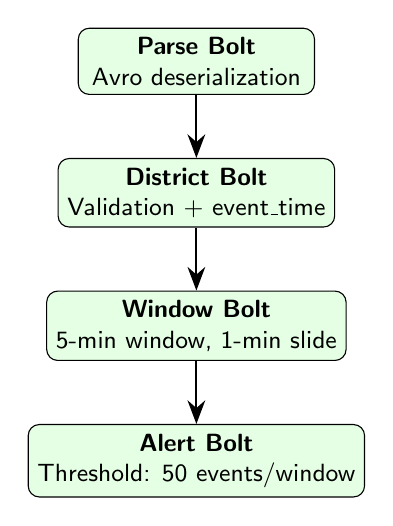
\begin{tikzpicture}[
  node distance=0.8cm,
  bolt/.style={rectangle, draw, rounded corners, fill=green!10, minimum width=3cm, minimum height=0.8cm, align=center, font=\small\sffamily},
  arr/.style={-{Stealth[length=3mm]}, thick},
]
\node[bolt] (parse) {\textbf{Parse Bolt}\\Avro deserialization};
\node[bolt, below=of parse] (district) {\textbf{District Bolt}\\Validation + event\_time};
\node[bolt, below=of district] (window) {\textbf{Window Bolt}\\5-min window, 1-min slide};
\node[bolt, below=of window] (alert) {\textbf{Alert Bolt}\\Threshold: 50 events/window};

\draw[arr] (parse) -- (district);
\draw[arr] (district) -- (window);
\draw[arr] (window) -- (alert);
\end{tikzpicture}
\caption{BoltPipeline four-stage processing}
\end{figure}

\subsubsection{Volume Threshold Alert Severity}

\begin{table}[H]
\centering
\caption{BoltPipeline alert severity levels}
\begin{tabular}{l l l}
\toprule
\textbf{Level} & \textbf{Condition} & \textbf{Example (threshold=50)} \\
\midrule
CRITICAL & count $>$ threshold $\times$ 3 & $>$ 150 events/window \\
HIGH & count $>$ threshold $\times$ 2 & $>$ 100 events/window \\
MEDIUM & count $>$ threshold & $>$ 50 events/window \\
\bottomrule
\end{tabular}
\end{table}

Volume alerts are written to PostgreSQL (\texttt{alerts} table), MongoDB (\texttt{whitechristmas.alert\_logs}), and the \texttt{anomaly-alerts} Kafka topic.

\subsection{Spark Configuration}

\begin{table}[H]
\centering
\caption{Spark Structured Streaming configuration}
\begin{tabular}{l l}
\toprule
\textbf{Parameter} & \textbf{Value} \\
\midrule
Window duration & 5 minutes (configurable) \\
Slide interval & 1 minute (configurable) \\
Watermark & 10 minutes (late data tolerance) \\
Anomaly threshold & 50 events/window (configurable) \\
Trigger interval & 30 seconds (ProcessingTime) \\
Checkpoint location & \texttt{/tmp/spark-checkpoint/} \\
JVM heap & 4 GB (G1GC) \\
Scala version & 2.13.16, Spark 4.0.1 \\
\bottomrule
\end{tabular}
\end{table}

% ============================================================================
% 7. BATCH ANALYTICS
% ============================================================================
\section{Batch Analytics Layer (Scala + Spark)}

\subsection{Overview}

The \texttt{BatchAnalytics} job runs on-demand to compute historical aggregations across the full CSV datasets. Unlike the streaming layer which processes events incrementally, the batch layer reads entire datasets and produces comprehensive analytical tables written to PostgreSQL in overwrite mode.

\subsection{Analytical Computations}

\subsubsection{Crime Trend Analysis}

Aggregates crime counts across four temporal dimensions (year, month, day of week, hour), enabling multi-granularity trend analysis. Output table: \texttt{crime\_trends}.

\subsubsection{Arrest Rate Analysis}

Performs a left join between Crimes and Arrests on \texttt{Case Number}, computing arrest rates by crime type, district, and race. A minimum threshold of 100 crimes filters statistically insignificant categories. Output tables: \texttt{arrest\_rate\_analysis}, \texttt{top\_arrest\_rate\_crime\_types}.

\subsubsection{Violence \& Gunshot Analysis}

Analyzes the Violence Reduction dataset for homicide detection (keyword matching on ``HOMICIDE''), non-fatal shooting identification, and gunshot proportion computation. Output tables: \texttt{violence\_analysis}, \texttt{top\_violence\_community}.

\subsubsection{Sex Offender Proximity Analysis}

Flags offenders with minor victims as ``PRIORITY'' and computes per-district offender density by joining with police station locations. Output tables: \texttt{sex\_offender\_proximity}, \texttt{district\_offender\_density}.

\subsubsection{K-Means Hotspot Detection}

\noindent\fbox{\parbox{\dimexpr\textwidth-2\fboxsep-2\fboxrule}{%
\textbf{K-Means Crime Hotspot Clustering}

Applies K-Means clustering ($k=10$, configurable) on crime latitude/longitude coordinates to identify geographic crime hotspots. For each cluster, the algorithm outputs:
\begin{itemize}
  \item Cluster centroid coordinates (latitude, longitude)
  \item Crime count within cluster
  \item Distribution of crime types (primary\_types)
\end{itemize}
This provides a data-driven alternative to manual precinct boundary analysis.
}}

Output table: \texttt{hotspots}.

\subsubsection{Cross-Dataset Correlation}

Computes two types of district/community-level correlations:
\begin{enumerate}
  \item \textbf{Violence rate vs.\ arrest rate} by CPD district
  \item \textbf{Sex offender density vs.\ crime rate} by community area
\end{enumerate}
Output table: \texttt{correlations}.

\subsection{Output Summary}

\begin{table}[H]
\centering
\caption{Batch analytics PostgreSQL output tables}
\label{tab:batch}
\begin{tabularx}{\textwidth}{l X}
\toprule
\textbf{Table} & \textbf{Contents} \\
\midrule
\texttt{crime\_trends} & Year/month/day/hour crime count aggregations \\
\texttt{arrest\_rate\_analysis} & Arrest rates by type, district, race \\
\texttt{top\_arrest\_rate\_crime\_types} & Top 10 crime types by arrest rate ($\geq$100 crimes) \\
\texttt{violence\_analysis} & Monthly homicide/shooting counts by district \\
\texttt{top\_violence\_community} & Top 20 communities by violence incidence \\
\texttt{sex\_offender\_proximity} & Offender demographics with priority flags \\
\texttt{district\_offender\_density} & Per-district offender counts \\
\texttt{hotspots} & K-Means cluster centroids with crime distribution \\
\texttt{correlations} & Violence-arrest and offender-crime correlations \\
\bottomrule
\end{tabularx}
\end{table}

% ============================================================================
% 8. REAL-TIME SERVING LAYER (GO)
% ============================================================================
\section{Real-Time Serving Layer (Go)}

\subsection{Overview}

The Go API service (\texttt{whitechristmas-api}) is the central serving layer, built with Chi router for HTTP and Gorilla WebSocket for real-time event delivery. It connects to Kafka (consumer), PostgreSQL (analytics queries), and MongoDB (alert retrieval), exposing both REST and WebSocket endpoints on port 8081.

\subsection{Kafka Consumer Architecture}

The API runs one goroutine per alert topic, each with an independent consumer group:

\begin{lstlisting}[caption={Multi-topic Kafka consumer initialization}]
topics := []string{
  "alerts-crimes", "alerts-violence",
  "alerts-arrests", "alerts-sex-offenders",
}
for _, topic := range topics {
  go consumeTopic(topic, hub) // independent goroutine
}
\end{lstlisting}

Each consumer reads JSON-serialized \texttt{CrimeEvent} messages, increments Prometheus counters, and broadcasts to all connected WebSocket clients through the \texttt{EventHub}.

\subsection{EventHub (WebSocket Pub/Sub)}

The \texttt{EventHub} is a thread-safe, channel-based pub/sub system:

\begin{figure}[H]
\centering
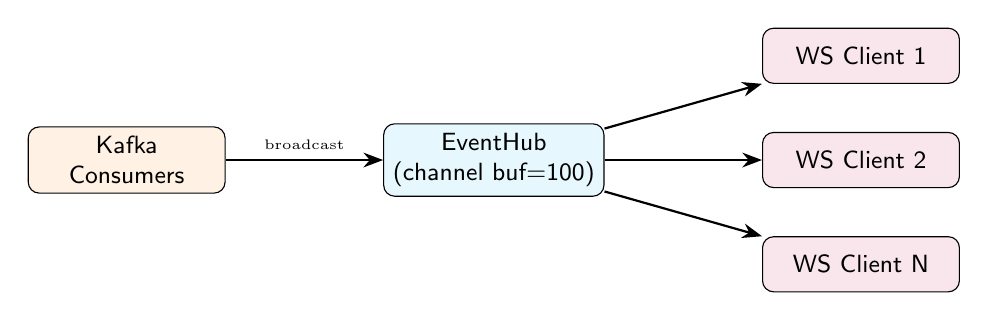
\begin{tikzpicture}[
  node distance=1cm and 2cm,
  block/.style={rectangle, draw, rounded corners, minimum width=2.5cm, minimum height=0.7cm, align=center, font=\small\sffamily},
  arr/.style={-{Stealth[length=2.5mm]}, thick},
]
\node[block, fill=orange!10] (kafka) {Kafka\\Consumers};
\node[block, fill=cyan!10, right=2cm of kafka] (hub) {EventHub\\(channel buf=100)};
\node[block, fill=purple!10, above right=0.5cm and 2cm of hub] (ws1) {WS Client 1};
\node[block, fill=purple!10, right=2cm of hub] (ws2) {WS Client 2};
\node[block, fill=purple!10, below right=0.5cm and 2cm of hub] (ws3) {WS Client N};

\draw[arr] (kafka) -- node[above, font=\tiny] {broadcast} (hub);
\draw[arr] (hub) -- (ws1);
\draw[arr] (hub) -- (ws2);
\draw[arr] (hub) -- (ws3);
\end{tikzpicture}
\caption{EventHub WebSocket broadcast architecture}
\end{figure}

\subsection{REST API Endpoints}

\begin{table}[H]
\centering
\caption{Go API REST endpoints}
\label{tab:api}
\begin{tabularx}{\textwidth}{l l X}
\toprule
\textbf{Endpoint} & \textbf{Source} & \textbf{Description} \\
\midrule
\texttt{GET /health} & --- & Service health check \\
\texttt{GET /stats} & Memory & Connected clients, total events \\
\texttt{GET /metrics} & Prometheus & Application metrics (OpenMetrics) \\
\midrule
\texttt{GET /events/history} & PostgreSQL & Paginated event history (limit, offset, dataset) \\
\texttt{GET /districts/summary} & PostgreSQL & Per-district counts, avg severity \\
\texttt{GET /datasets/summary} & PostgreSQL & Per-dataset counts, avg severity, critical events \\
\midrule
\texttt{GET /analytics/trends} & PostgreSQL & Hourly event counts (configurable hours) \\
\texttt{GET /analytics/crime-trends} & PostgreSQL & Monthly crime aggregations \\
\texttt{GET /analytics/hotspots} & PostgreSQL & K-Means cluster centroids \\
\texttt{GET /analytics/correlations} & PostgreSQL & District/community correlation data \\
\texttt{GET /analytics/arrest-rates} & PostgreSQL & Crime type arrest rates \\
\texttt{GET /analytics/violence} & PostgreSQL & Monthly homicide/shooting statistics \\
\texttt{GET /analytics/sex-offenders} & PostgreSQL & Offender demographics and priority counts \\
\texttt{GET /analytics/severity} & PostgreSQL & Event severity distribution \\
\midrule
\texttt{GET /alerts/recent} & MongoDB & Recent alerts (sorted by timestamp) \\
\texttt{GET /ws} & Kafka & WebSocket real-time event stream \\
\bottomrule
\end{tabularx}
\end{table}

\subsection{Database Initialization}

The Go API auto-creates all required PostgreSQL tables at startup (\texttt{initPostgres}), including: \texttt{events}, \texttt{alerts}, \texttt{crime\_trends}, \texttt{top\_arrest\_rate\_crime\_types}, \texttt{violence\_analysis}, \texttt{hotspots}, \texttt{correlations}, \texttt{sex\_offender\_proximity}, and \texttt{district\_offender\_density}. Connection pool: 10 max open, 5 idle, 5-minute lifetime.

\subsection{Graceful Degradation}

Both PostgreSQL and MongoDB connections are optional. If unavailable, the API continues to function with real-time WebSocket delivery from Kafka, returning 503 for database-backed endpoints. This ensures the live event stream remains operational even during database maintenance.

% ============================================================================
% 9. STORAGE LAYER
% ============================================================================
\section{Storage Layer}

\subsection{Dual-Model Persistence}

WhiteChristmas uses a dual-database strategy, selecting the optimal storage model for each data type:

\begin{table}[H]
\centering
\caption{Storage model selection}
\begin{tabularx}{\textwidth}{l X X}
\toprule
\textbf{Database} & \textbf{Use Case} & \textbf{Rationale} \\
\midrule
PostgreSQL 16 & Structured analytics, aggregations, time-series, relational joins & SQL queries for complex analytical joins (arrest rates, correlations), ACID transactions for event consistency \\
MongoDB 7.0 & Alert logs, flexible event storage, recent alerts cache & Schema-flexible documents for semi-structured alerts, fast timestamp-sorted retrieval \\
\bottomrule
\end{tabularx}
\end{table}

\subsection{PostgreSQL Schema}

PostgreSQL stores both streaming output (from Spark) and batch analytics results:

\textbf{Streaming tables:}
\begin{itemize}
  \item \texttt{events} --- All processed events (append-only, indexed on \texttt{source\_dataset}, \texttt{processed\_at})
  \item \texttt{alerts} --- Volume anomaly alerts from BoltPipeline
\end{itemize}

\textbf{Batch analytics tables:} 9 tables as detailed in Table~\ref{tab:batch}.

\subsection{MongoDB Collections}

\begin{itemize}
  \item \texttt{whitechristmas.alerts} --- Severity-based alerts from StreamProcessor (severity $\geq$ 3)
  \item \texttt{whitechristmas.alert\_logs} --- Volume anomaly alerts from BoltPipeline
\end{itemize}

% ============================================================================
% 10. FRONTEND
% ============================================================================
\section{Frontend Dashboard (Next.js)}

\subsection{Overview}

The frontend is a single-page Next.js 15 application (React 19) implementing a real-time crime analytics dashboard. It uses ECharts 6.0 for all data visualizations, Leaflet 1.9 for interactive mapping, and Tailwind CSS 4.0 for styling with a dark cyberpunk aesthetic.

\subsection{Dashboard Layout}

The dashboard is organized into five horizontal sections:

\begin{figure}[H]
\centering
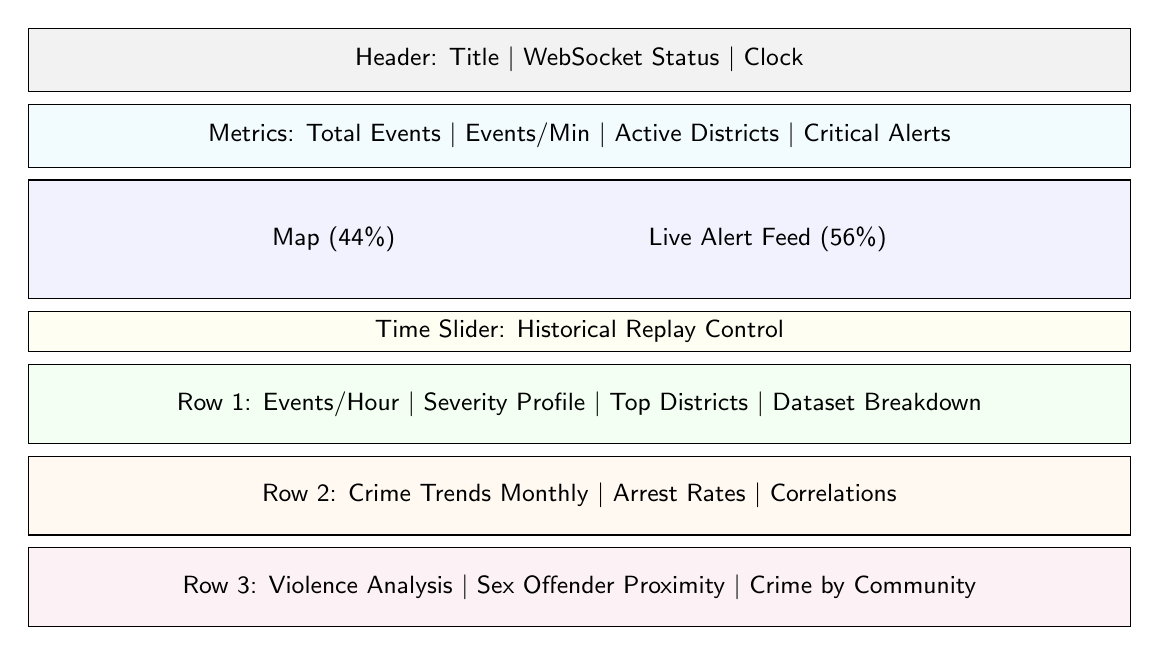
\begin{tikzpicture}[
  section/.style={rectangle, draw, minimum width=14cm, align=center, font=\small\sffamily},
]
\node[section, minimum height=0.8cm, fill=gray!10] (h) {Header: Title $\mid$ WebSocket Status $\mid$ Clock};
\node[section, minimum height=0.8cm, fill=cyan!5, below=0.15cm of h] (m) {Metrics: Total Events $\mid$ Events/Min $\mid$ Active Districts $\mid$ Critical Alerts};
\node[section, minimum height=1.5cm, fill=blue!5, below=0.15cm of m] (map) {Map (44\%) \hspace{3cm} Live Alert Feed (56\%)};
\node[section, minimum height=0.5cm, fill=yellow!5, below=0.15cm of map] (ts) {Time Slider: Historical Replay Control};
\node[section, minimum height=1cm, fill=green!5, below=0.15cm of ts] (r1) {Row 1: Events/Hour $\mid$ Severity Profile $\mid$ Top Districts $\mid$ Dataset Breakdown};
\node[section, minimum height=1cm, fill=orange!5, below=0.15cm of r1] (r2) {Row 2: Crime Trends Monthly $\mid$ Arrest Rates $\mid$ Correlations};
\node[section, minimum height=1cm, fill=purple!5, below=0.15cm of r2] (r3) {Row 3: Violence Analysis $\mid$ Sex Offender Proximity $\mid$ Crime by Community};
\end{tikzpicture}
\caption{Dashboard layout structure}
\end{figure}

\subsection{Visualizations}

The dashboard renders 10 distinct chart types:

\begin{table}[H]
\centering
\caption{Dashboard chart components}
\begin{tabularx}{\textwidth}{c l l l X}
\toprule
\textbf{\#} & \textbf{Chart} & \textbf{Type} & \textbf{Refresh} & \textbf{Data Source} \\
\midrule
1 & Events/Hour & Line + area & 30s & \texttt{/analytics/trends} \\
2 & Severity Profile & Donut pie & 30s & \texttt{/analytics/severity} \\
3 & Top Districts & Horiz.\ bar & 15s & \texttt{/districts/summary} \\
4 & Dataset Breakdown & Horiz.\ bar & 15s & \texttt{/datasets/summary} \\
5 & Crime Trends Monthly & Vert.\ bar & 5min & \texttt{/analytics/crime-trends} \\
6 & Arrest Rates & Horiz.\ bar & 5min & \texttt{/analytics/arrest-rates} \\
7 & Correlations & Grouped bar & 5min & \texttt{/analytics/correlations} \\
8 & Violence Analysis & Stacked bar & 5min & \texttt{/analytics/violence} \\
9 & Sex Offender & Horiz.\ bar & 5min & \texttt{/analytics/sex-offenders} \\
10 & Crime by Community & Horiz.\ bar & 5min & \texttt{/analytics/correlations} \\
\bottomrule
\end{tabularx}
\end{table}

\subsection{Interactive Map}

The Leaflet-based map component (\texttt{DistrictMap.tsx}) renders:
\begin{itemize}
  \item \textbf{Canvas heatmap overlay:} Additive blobs with severity-based coloring (red $\geq$4.5, orange $\geq$4.0, yellow $\geq$3.0, cyan $<$3.0)
  \item \textbf{District labels:} 26 CPD district centroids with monospace labels
  \item \textbf{Hotspot markers:} Crosshair-style pins at K-Means cluster centroids with crime type breakdown popups
  \item \textbf{Interactive popups:} District name, total events, average severity on click
\end{itemize}

\subsection{Real-Time Data Pipeline}

The frontend maintains two parallel data pipelines:

\begin{description}
  \item[WebSocket (live):] Connects to \texttt{ws://localhost:8081/ws}, receives typed messages (\texttt{event}, \texttt{stats}, \texttt{connection}), maintains a rolling buffer of 150 events.
  \item[REST polling:] 12 endpoints polled at intervals from 2s (stats) to 5min (batch analytics), using \texttt{fetch} with error handling and logging.
\end{description}

\subsection{Historical Replay}

The time slider component enables scrubbing through historical events. Moving the slider triggers a \texttt{GET /events/history?limit=50\&offset=X} request, replacing the live feed with historical data and displaying a ``PAUSED'' indicator.

\subsection{Dashboard Screenshot}

\begin{figure}[H]
\centering
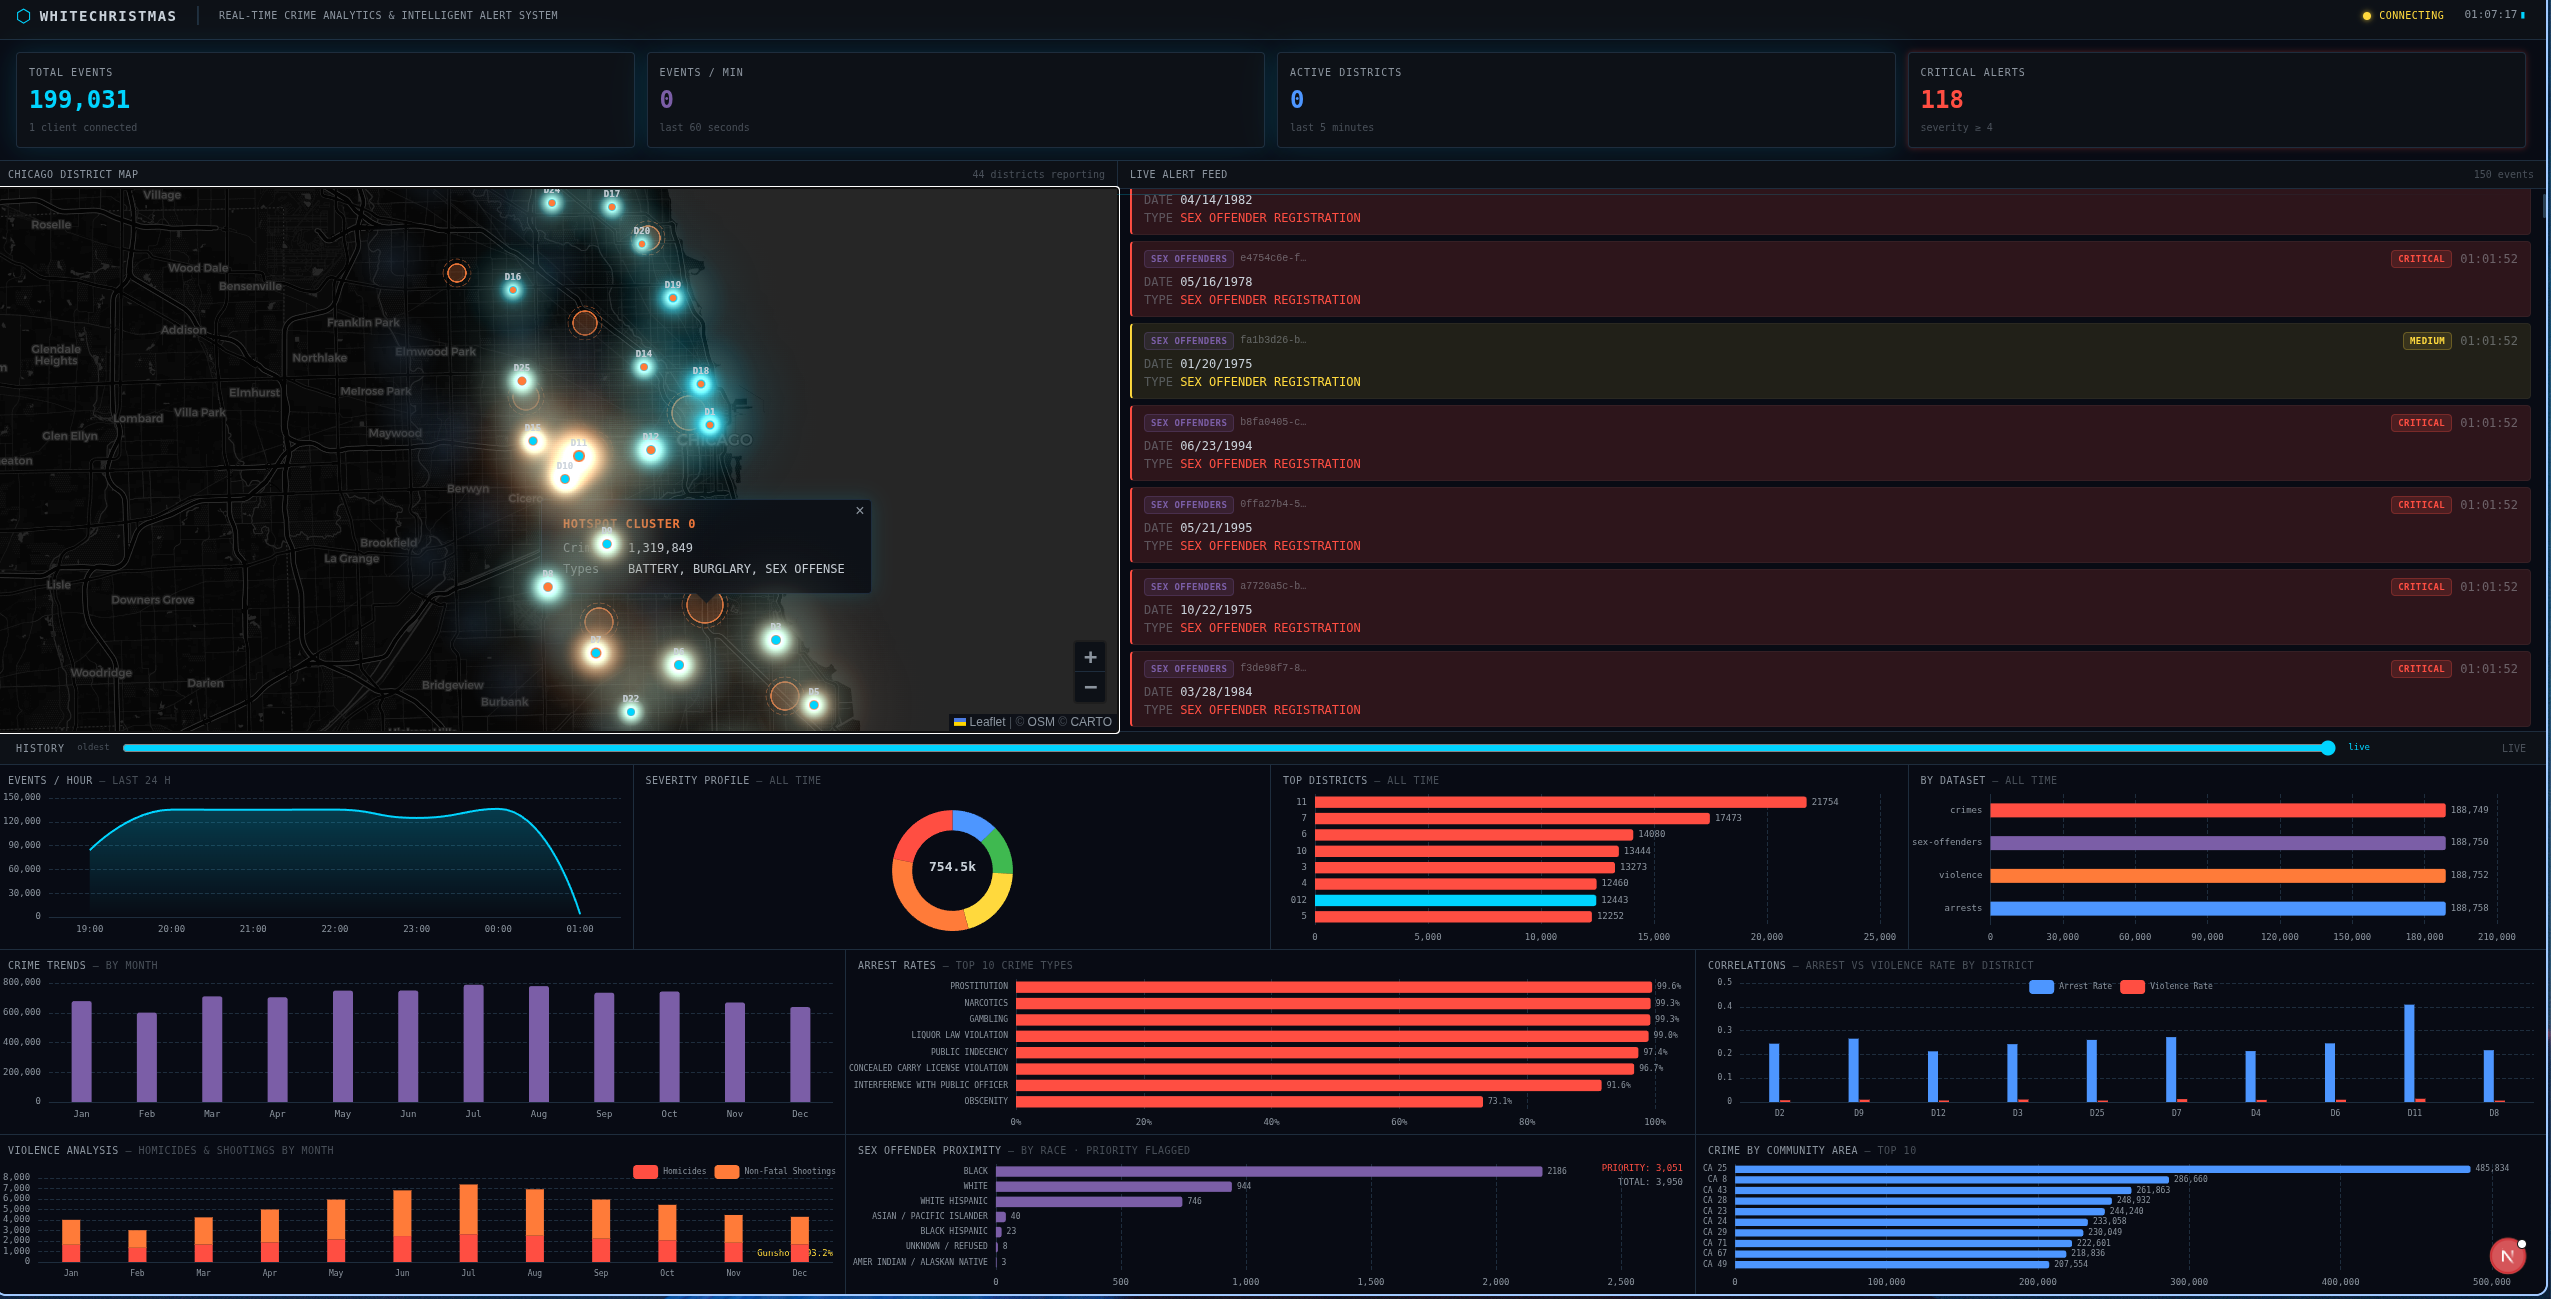
\includegraphics[width=\textwidth]{dashboard.png}
\caption{WhiteChristmas real-time crime analytics dashboard showing the interactive map with district heatmap overlay, live alert feed, KPI metrics, and multi-row chart panels}
\label{fig:dashboard}
\end{figure}

% ============================================================================
% 11. OBSERVABILITY
% ============================================================================
\section{Observability \& Monitoring}

\subsection{Prometheus Metrics}

The Go API exposes application metrics on \texttt{/metrics} in OpenMetrics format. Prometheus scrapes this endpoint every 5 seconds.

\begin{table}[H]
\centering
\caption{Application Prometheus metrics}
\label{tab:metrics}
\begin{tabularx}{\textwidth}{l l l X}
\toprule
\textbf{Metric} & \textbf{Type} & \textbf{Labels} & \textbf{Description} \\
\midrule
\texttt{events\_total} & Counter & severity, dataset & Total events broadcast \\
\texttt{websocket\_clients} & Gauge & --- & Active WebSocket connections \\
\texttt{kafka\_messages\_total} & Counter & topic & Kafka messages consumed \\
\texttt{http\_request\_duration\_seconds} & Histogram & method, route, status & Request latency \\
\texttt{broadcast\_errors\_total} & Counter & --- & Failed WebSocket writes \\
\bottomrule
\end{tabularx}
\end{table}

\subsection{Alert Rules}

Seven Prometheus alerting rules monitor system health:

\begin{table}[H]
\centering
\caption{Prometheus alert rules}
\begin{tabularx}{\textwidth}{l l l X}
\toprule
\textbf{Alert} & \textbf{Severity} & \textbf{For} & \textbf{Condition} \\
\midrule
APIDown & Critical & 30s & API target unreachable \\
NoEventsIngested & Warning & 3min & Zero event rate for 2+ minutes \\
LowEventRate & Info & 5min & $<$0.5 events/sec over 5 minutes \\
HighBroadcastErrors & Warning & 1min & $>$0.1 errors/sec \\
HighHTTP5xx & Warning & 2min & $>$5\% of requests returning 5xx \\
HighAPILatency & Warning & 5min & P99 latency $>$2 seconds \\
DatasetIngestStopped & Warning & 5min & No events from specific dataset \\
\bottomrule
\end{tabularx}
\end{table}

\subsection{Grafana Dashboards}

Two pre-provisioned Grafana dashboards (port 3001) provide operational visibility:

\begin{itemize}
  \item \textbf{WhiteChristmas Pipeline:} 14 panels covering event ingestion rates (by severity and dataset), Kafka consumption by topic, HTTP request rates, P99 latency by route, WebSocket client count, per-dataset event counters, and broadcast errors.
  \item \textbf{Pipeline Metrics:} Focused view on events total, active WebSocket clients, Kafka messages consumed, broadcast errors, events/second by severity, and HTTP latency (p99).
\end{itemize}

\begin{figure}[H]
\centering
\begin{subfigure}[b]{0.48\textwidth}
  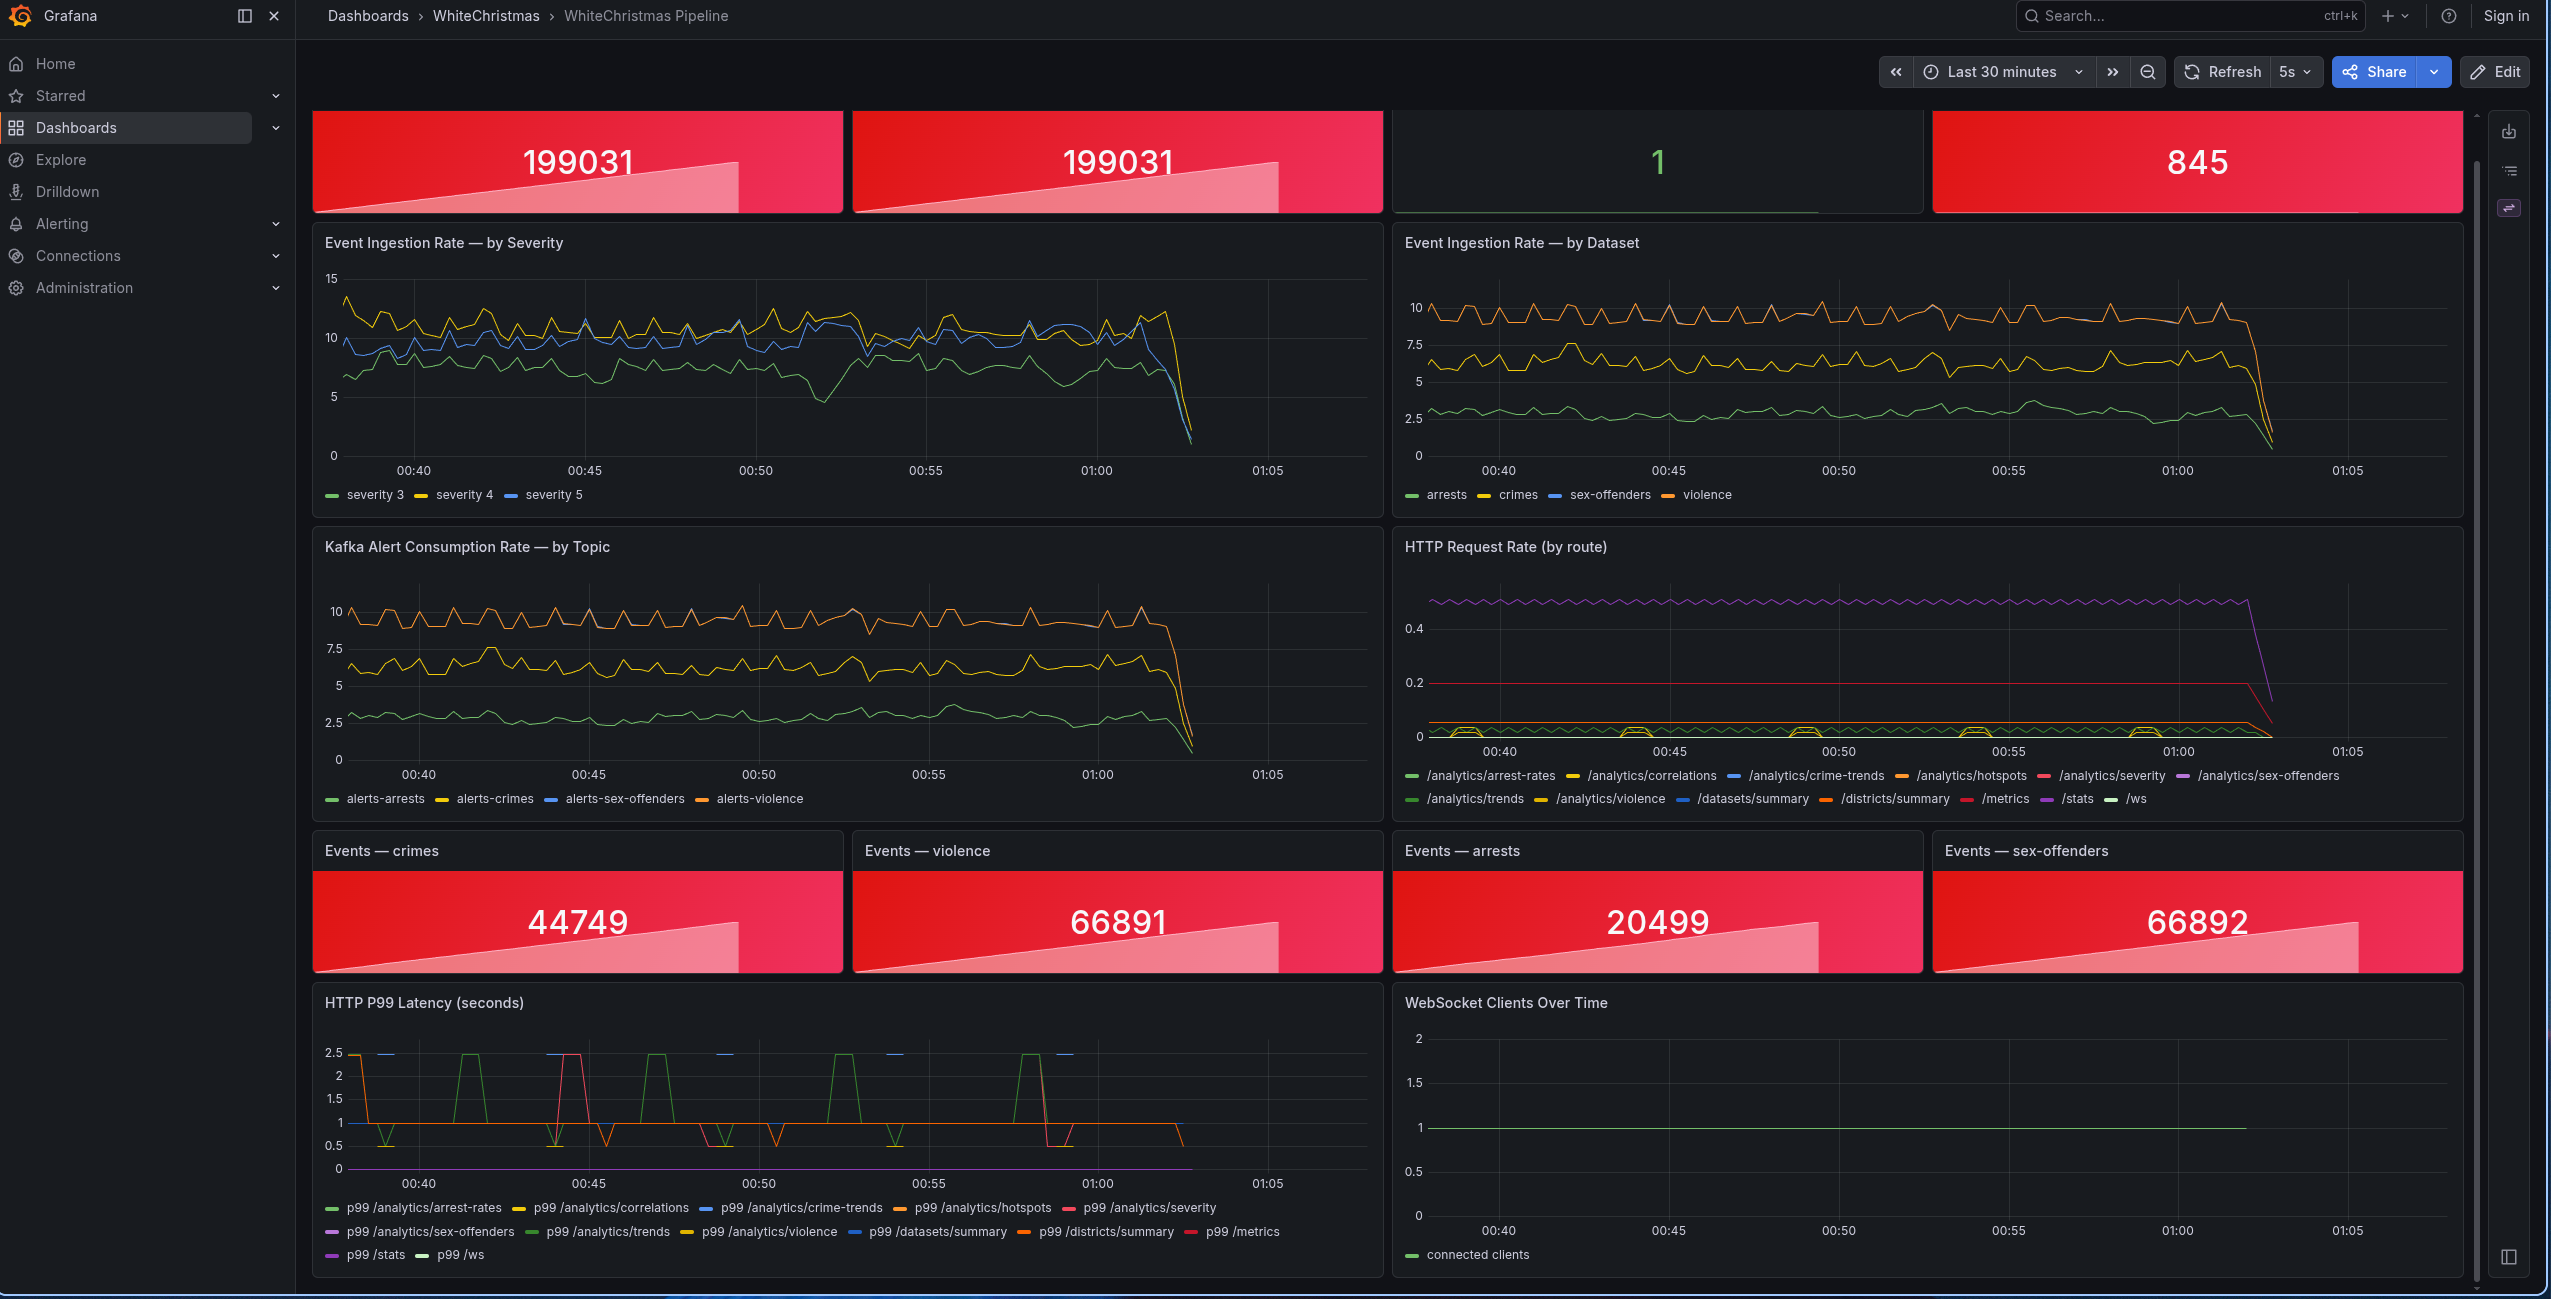
\includegraphics[width=\textwidth]{grafana.png}
  \caption{Main Grafana dashboard}
  \label{fig:grafana}
\end{subfigure}
\hfill
\begin{subfigure}[b]{0.48\textwidth}
  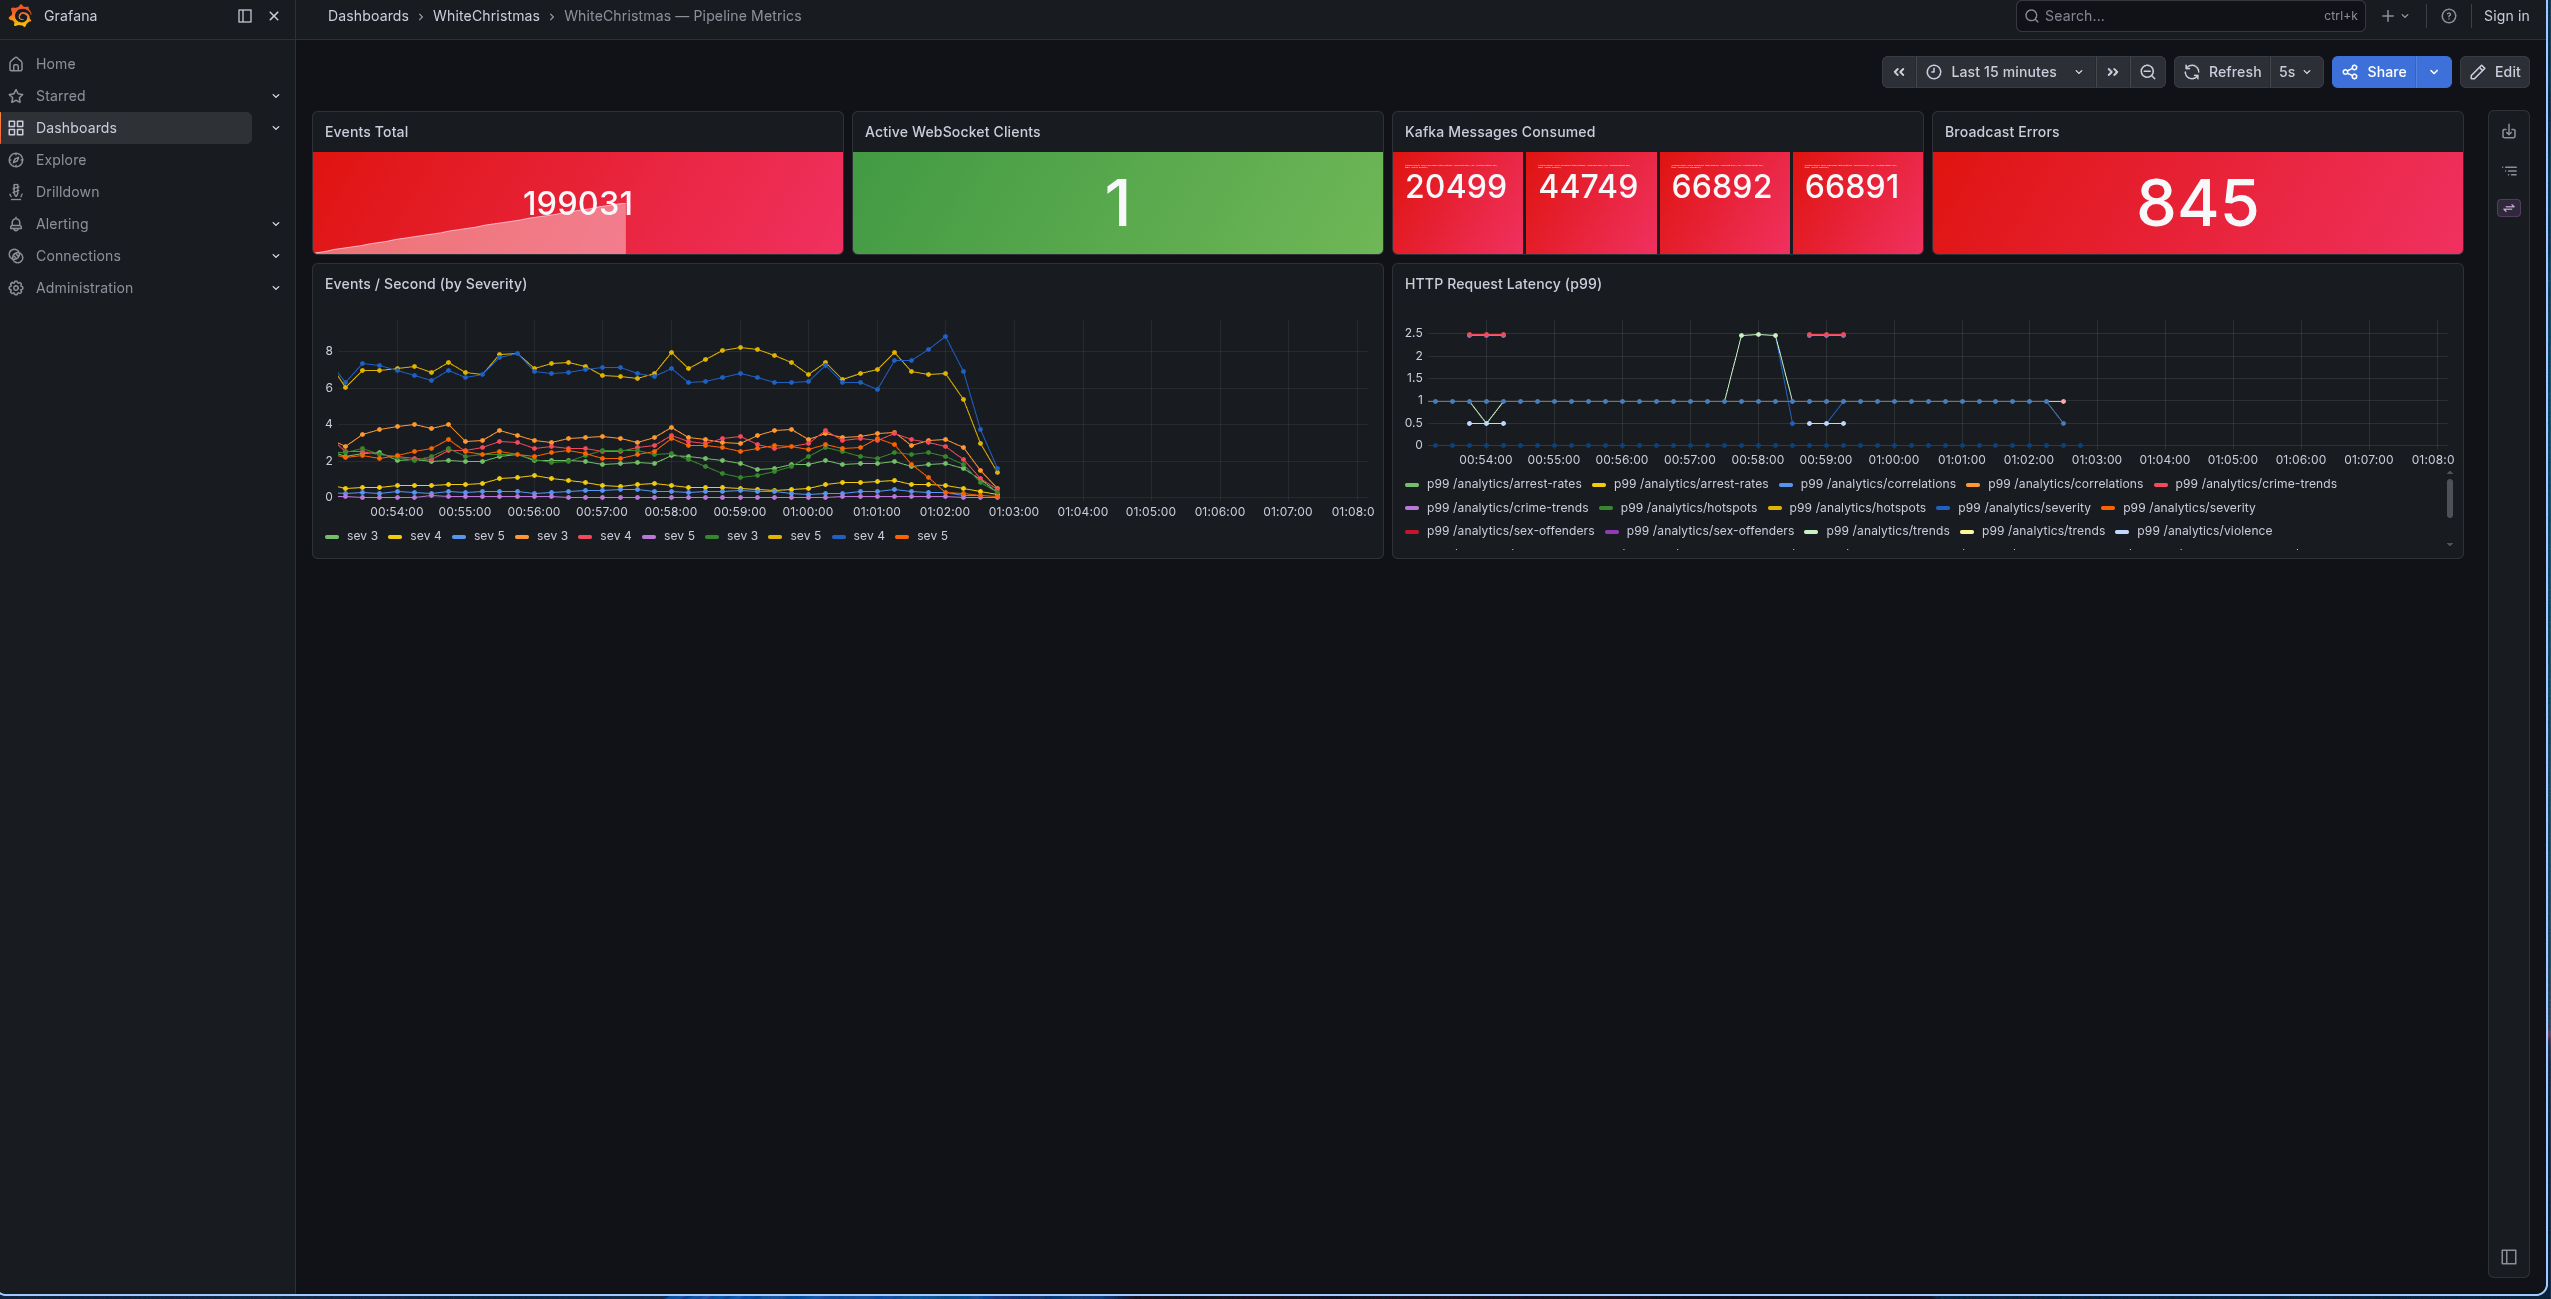
\includegraphics[width=\textwidth]{grafana-metrics-pipeline.png}
  \caption{Pipeline metrics dashboard}
  \label{fig:grafana-metrics}
\end{subfigure}
\caption{Grafana observability dashboards showing event ingestion rates, Kafka consumption, HTTP latency, and WebSocket client metrics}
\end{figure}

\begin{figure}[H]
\centering
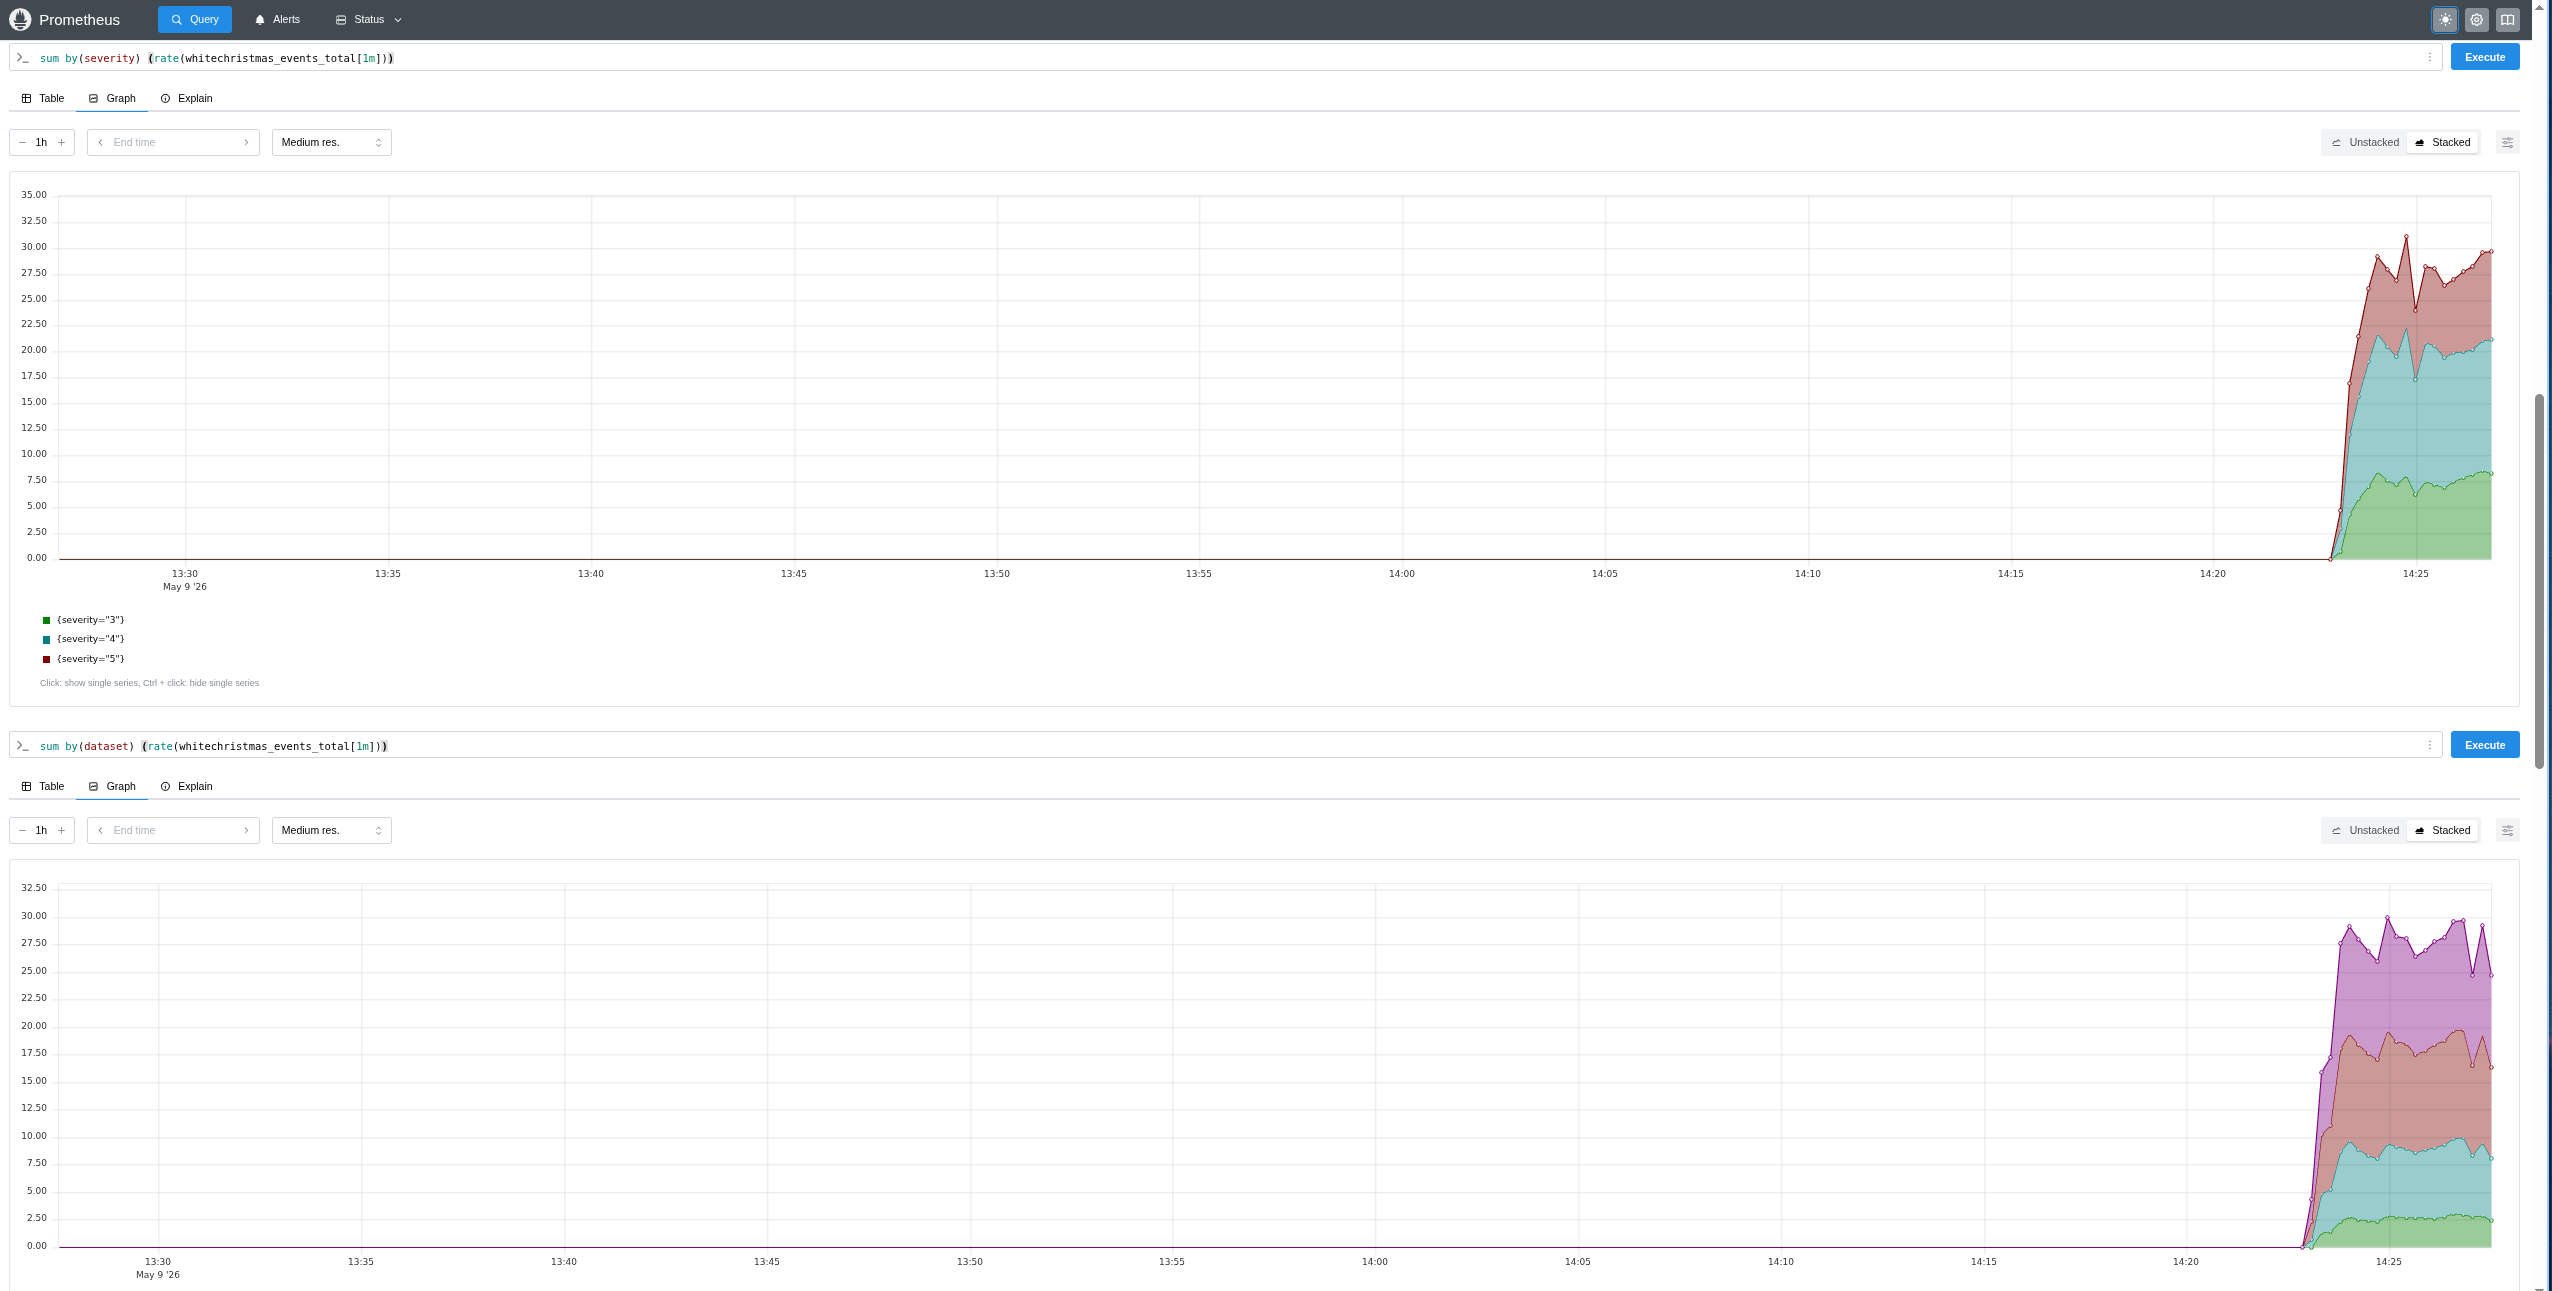
\includegraphics[width=\textwidth]{prometheus.png}
\caption{Prometheus query interface showing event rate by severity (top) and by dataset (bottom), demonstrating the multi-dimensional metrics collection}
\label{fig:prometheus}
\end{figure}

% ============================================================================
% 12. INFRASTRUCTURE & DEPLOYMENT
% ============================================================================
\section{Infrastructure \& Deployment}

\subsection{Docker Compose Architecture}

The entire platform is orchestrated via Docker Compose with 12 services:

\begin{table}[H]
\centering
\caption{Docker Compose service inventory}
\begin{tabularx}{\textwidth}{l l c X}
\toprule
\textbf{Service} & \textbf{Image} & \textbf{Port} & \textbf{Role} \\
\midrule
\texttt{wc-kafka} & Confluent 7.7.0 & 9092/29092 & KRaft message broker \\
\texttt{wc-schema-registry} & Confluent 7.7.0 & 8082 & Avro schema management \\
\texttt{kafka-init} & Confluent 7.7.0 & --- & Topic creation (run-once) \\
\texttt{wc-postgres} & PostgreSQL 16 & 5432 & Relational analytics store \\
\texttt{wc-mongodb} & MongoDB 7.0 & 27017 & Document alert store \\
\texttt{wc-spark-streaming} & Custom (JDK 21) & --- & StreamProcessor + BoltPipeline \\
\texttt{wc-producer} & Custom (Rust) & --- & CSV $\rightarrow$ Kafka ingestion \\
\texttt{wc-batch-analytics} & Custom (JDK 21) & --- & Historical analytics (on-demand) \\
\texttt{wc-api} & Custom (Go) & 8081 & REST + WebSocket API \\
\texttt{wc-frontend} & Custom (Node.js) & 3000 & Next.js dashboard \\
\texttt{wc-prometheus} & Prometheus 2.54 & 9090 & Metrics collection \\
\texttt{wc-grafana} & Grafana 11.2 & 3001 & Metrics visualization \\
\bottomrule
\end{tabularx}
\end{table}

\subsection{Service Dependency Graph}

\begin{figure}[H]
\centering
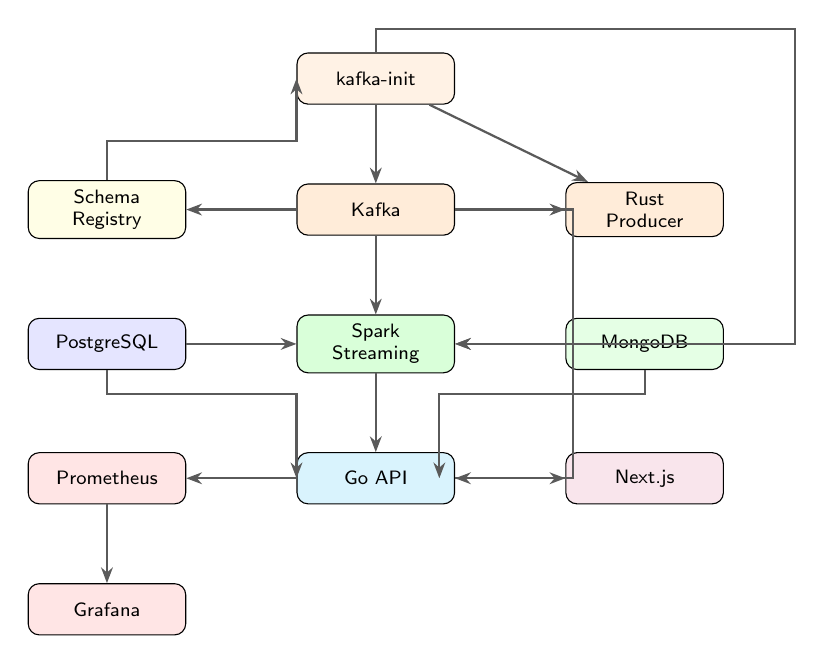
\begin{tikzpicture}[
  node distance=1cm and 1.4cm,
  svc/.style={rectangle, draw, rounded corners, minimum width=2.0cm, minimum height=0.65cm, align=center, font=\scriptsize\sffamily},
  arr/.style={-{Stealth[length=2mm]}, thick, color=codegray},
]
% Top: kafka-init
\node[svc, fill=orange!10] (init) {kafka-init};

% Center row: Kafka with Schema Registry left and Rust Producer right
\node[svc, fill=orange!15, below=of init] (kafka) {Kafka};
\node[svc, fill=yellow!10, left=of kafka] (sr) {Schema\\Registry};
\node[svc, fill=orange!15, right=of kafka] (producer) {Rust\\Producer};

% Center: Spark Streaming with PostgreSQL left and MongoDB right
\node[svc, fill=green!15, below=of kafka] (spark) {Spark\\Streaming};
\node[svc, fill=blue!10, left=of spark] (pg) {PostgreSQL};
\node[svc, fill=green!10, right=of spark] (mongo) {MongoDB};

% Below spark: Go API
\node[svc, fill=cyan!15, below=of spark] (api) {Go API};

% Bottom row: Prometheus left of api, Next.js right of api
\node[svc, fill=red!10, left=of api] (prom) {Prometheus};
\node[svc, fill=purple!10, right=of api] (fe) {Next.js};

% Grafana below Prometheus
\node[svc, fill=red!10, below=of prom] (graf) {Grafana};

% Direct, short arrows
\draw[arr] (init) -- (kafka);
\draw[arr] (kafka) -- (sr);
\draw[arr] (kafka) -- (producer);
\draw[arr] (kafka) -- (spark);
\draw[arr] (pg) -- (spark);
\draw[arr] (mongo) -- (spark);
\draw[arr] (spark) -- (api);
\draw[arr] (api) -- (fe);
\draw[arr] (api) -- (prom);
\draw[arr] (prom) -- (graf);

% Routed arrows that would otherwise cross nodes
% sr -> init: up from sr.north, then over to init.west
\draw[arr] (sr.north) -- ++(0,0.5) -| (init.west);
% init -> producer: simple diagonal (clears kafka because init sits directly above)
\draw[arr] (init) -- (producer);
% init -> spark: out the right gutter (far), down past producer/mongo, into spark.east
\draw[arr] (init.north) -- ++(0,0.3) -| ($(mongo.east)+(0.9,0)$) |- (spark.east);
% kafka -> api: out the right gutter (closer), down past spark/mongo, into api.east
\draw[arr] (kafka.east) -- ++(1.5,0) |- (api.east);
% pg -> api: drop below pg, then over to api.west
\draw[arr] (pg.south) -- ++(0,-0.3) -| (api.west);
% mongo -> api: drop below mongo, then over to api.east (slightly inset to avoid kafka->api line)
\draw[arr] (mongo.south) -- ++(0,-0.3) -| ($(api.east)+(-0.2,0)$);
\end{tikzpicture}
\caption{Service dependency graph}
\end{figure}

\subsection{Volume Persistence}

Four named Docker volumes ensure data persistence across restarts:
\begin{itemize}
  \item \texttt{postgres\_data} --- PostgreSQL databases
  \item \texttt{mongodb\_data} --- MongoDB collections
  \item \texttt{prometheus\_data} --- 7-day metrics retention
  \item \texttt{spark\_checkpoint} --- Spark streaming checkpoints
\end{itemize}

\subsection{Native Development Environment}

For local development without Docker, the project provides shell scripts for starting/stopping each infrastructure component (Kafka, Schema Registry, Prometheus, Grafana) with NixOS integration via \texttt{shell.nix}/\texttt{flake.nix}.

% ============================================================================
% 13. ML APPROACH
% ============================================================================
\section{Machine Learning \& Statistical Methods}

\subsection{Design Philosophy}

WhiteChristmas deliberately favors \textbf{simple, explainable statistical methods} over complex ML pipelines. This decision was driven by:
\begin{itemize}
  \item \textbf{Explainability:} Statistical methods produce interpretable results that can be communicated to non-technical stakeholders
  \item \textbf{Debuggability:} Z-scores and thresholds are transparent --- anomalies can be traced to specific numerical conditions
  \item \textbf{Latency:} Statistical computations operate within Spark's streaming micro-batch model without requiring model inference
  \item \textbf{Reliability:} No model drift, no training pipeline, no feature store complexity
\end{itemize}

\subsection{Z-Score Anomaly Detection}

The primary anomaly detection method uses z-score analysis within sliding windows:

\begin{align}
\text{For window } W \text{ grouped by district:} \nonumber \\
\mu_W &= \frac{1}{|W|} \sum_{e \in W} \text{severity}(e) \\
\sigma_W &= \sqrt{\frac{1}{|W|} \sum_{e \in W} (\text{severity}(e) - \mu_W)^2} \\
z &= \frac{\max_{e \in W}(\text{severity}(e)) - \mu_W}{\sigma_W} \\
\text{Anomaly} &\iff z > 2.0
\end{align}

Window parameters: 2-minute tumbling windows with 30-second slides, grouped by district.

\subsection{Volume Threshold Detection}

The BoltPipeline uses absolute count thresholds within sliding windows. For 5-minute windows with 1-minute slides, grouped by \texttt{(dataset, district)}:

\begin{align}
\text{count}_W &= |\{e \in W\}| \\
\text{Alert severity} &= \begin{cases}
  \text{CRITICAL} & \text{count}_W > 3\theta \\
  \text{HIGH} & \text{count}_W > 2\theta \\
  \text{MEDIUM} & \text{count}_W > \theta
\end{cases}
\end{align}

where $\theta = 50$ (configurable via \texttt{ANOMALY\_THRESHOLD}).

\subsection{K-Means Geographic Clustering}

Spark MLlib's K-Means algorithm identifies crime hotspots:

\begin{itemize}
  \item \textbf{Features:} (latitude, longitude) from crimes dataset
  \item \textbf{K:} 10 clusters (configurable via \texttt{KMEANS\_K})
  \item \textbf{Output:} Cluster centroids with associated crime counts and type distributions
  \item \textbf{Application:} Hotspot markers rendered on the Leaflet map with crosshair pins
\end{itemize}

\subsection{Severity Scoring Model}

Each dataset applies a rule-based severity classifier mapping domain knowledge to a 1--5 integer scale. The rules encode criminological severity hierarchies (e.g., homicide $>$ assault $>$ theft) and legal classification systems (e.g., felony classes X $>$ 1 $>$ 2 $>$ A for arrests).

% ============================================================================
% 14. RESULTS
% ============================================================================
\section{Results}

\subsection{System Performance}

During live pipeline execution, the system processed the following volumes:

\begin{table}[H]
\centering
\caption{Pipeline throughput metrics (observed)}
\label{tab:results}
\begin{tabular}{l r}
\toprule
\textbf{Metric} & \textbf{Value} \\
\midrule
Total events ingested & 199,031 \\
Kafka messages consumed & 199,031 \\
Active WebSocket clients & 1 (dashboard) \\
Broadcast errors & 845 \\
\midrule
Events --- crimes & 44,749 \\
Events --- violence & 66,891 \\
Events --- arrests & 20,499 \\
Events --- sex-offenders & 66,892 \\
\bottomrule
\end{tabular}
\end{table}

\subsection{Event Distribution by Severity}

The severity distribution across all processed events shows the expected long-tail pattern, with the majority of events at lower severity levels and a significant proportion of high-severity events from the violence and sex-offender datasets.

\begin{table}[H]
\centering
\caption{Severity distribution from dashboard observations}
\begin{tabular}{l l l}
\toprule
\textbf{Severity} & \textbf{Label} & \textbf{Color Code} \\
\midrule
5 & CRITICAL & Red --- Homicides, Class X felonies, minor victims \\
4 & HIGH & Orange --- Shootings, assault, battery, Class 1-2 felonies \\
3 & MEDIUM & Yellow --- Theft, burglary, Class 3-4 felonies, default sex offender \\
2 & LOW & Green --- Deceptive practice, fraud, Class A misdemeanors \\
1 & INFO & Blue --- Minor offenses, default \\
\bottomrule
\end{tabular}
\end{table}

\subsection{Batch Analytics Results}

\subsubsection{Crime Trends}

The batch analytics job produces monthly crime count aggregations spanning 2001--present, revealing seasonal patterns (summer peaks) and long-term trends (declining crime rates post-2016).

\subsubsection{Arrest Rates by Crime Type}

The top 10 crime types by arrest rate (minimum 100 crimes) are displayed on the dashboard, with color coding indicating rate severity: red ($>$50\%), yellow ($>$25\%), green ($\leq$25\%).

\subsubsection{Violence Analysis}

Monthly homicide and non-fatal shooting counts are displayed as stacked bar charts with gunshot proportion overlays, enabling temporal pattern identification.

\subsubsection{K-Means Hotspot Clusters}

The 10 identified crime hotspots are rendered as interactive markers on the Leaflet map, with popup details showing per-cluster crime count and type distribution.

\subsubsection{Cross-Dataset Correlations}

District-level correlations between arrest rates and violence rates are visualized as grouped bar charts, revealing districts with disproportionate violence-to-arrest ratios.

\subsection{Observability Results}

The Grafana dashboards (Figures~\ref{fig:grafana} and~\ref{fig:grafana-metrics}) demonstrate:
\begin{itemize}
  \item Steady event ingestion rates across all four datasets
  \item HTTP request rates by route showing analytics endpoint usage patterns
  \item P99 latency consistently below 1 second for all API routes
  \item WebSocket client connectivity tracking
  \item Per-severity event rate breakdown (Figure~\ref{fig:prometheus})
\end{itemize}

% ============================================================================
% 15. CHALLENGES
% ============================================================================
\section{Challenges \& Lessons Learned}

\subsection{Avro Deserialization Across Languages}

\textbf{Challenge:} The Confluent wire format prepends a 5-byte header (magic byte + 4-byte schema ID) before the Avro payload. Spark's built-in Avro deserializer does not handle this format natively.

\textbf{Solution:} Implemented manual header stripping in the Spark consumer using binary substring operations before passing the payload to the Avro deserializer. This required careful byte-level manipulation across the JVM/Scala boundary.

\subsection{Event-Time vs.\ Processing-Time Semantics}

\textbf{Challenge:} CSV replay simulates real-time streaming, but event timestamps span decades (2001--present). Using event-time windowing with historical timestamps causes watermark issues.

\textbf{Solution:} The BoltPipeline constructs \texttt{event\_time} from incident date/time with a fallback to the Kafka ingestion timestamp. A 10-minute watermark provides tolerance for out-of-order arrival without excessive state retention.

\subsection{Polyglot Schema Synchronization}

\textbf{Challenge:} Three languages (Rust, Scala, Go) must agree on a single event schema. Manual schema duplication risks drift.

\textbf{Solution:} A single \texttt{crime-event.avsc} file serves as the source of truth. The Rust producer reads and registers it; Spark loads it at runtime for deserialization; the Go API consumes the JSON-serialized alert format produced by Spark, which is derived from the same schema.

\subsection{WebSocket Connection Management}

\textbf{Challenge:} Go's goroutine model requires careful synchronization for the EventHub's client map, which is accessed from multiple goroutines (register, unregister, broadcast, stats queries).

\textbf{Solution:} Channel-based pub/sub with a dedicated \texttt{Run()} goroutine serializing all state mutations. An \texttt{RWMutex} protects the client count for concurrent reads from the stats endpoint.

\subsection{Spark Checkpoint Recovery}

\textbf{Challenge:} Spark Structured Streaming requires checkpoint directories for exactly-once guarantees. Docker volume mounts must persist checkpoints across container restarts.

\textbf{Solution:} A dedicated \texttt{spark\_checkpoint} volume maps to \texttt{/tmp/spark-checkpoint/} with separate subdirectories per query (\texttt{main}, \texttt{metrics}, \texttt{anomaly}, \texttt{alert-bolt}).

\subsection{Frontend Performance with High-Frequency Updates}

\textbf{Challenge:} At 40 events/second, naive React re-renders cause frame drops and browser resource exhaustion.

\textbf{Solution:} Event buffer capped at 150 items; canvas-based rendering for charts (ECharts) and map overlays (Leaflet); \texttt{ResizeObserver} instead of polling for responsive layout; tiered polling intervals (2s--5min) to reduce HTTP overhead.

\subsection{Docker Compose Service Ordering}

\textbf{Challenge:} Services have complex startup dependencies (Kafka must be healthy before Schema Registry, which must be healthy before producers/consumers).

\textbf{Solution:} Health checks on critical services (Kafka: \texttt{kafka-broker-api-versions}, Schema Registry: \texttt{curl /subjects}, PostgreSQL: \texttt{pg\_isready}) with \texttt{condition: service\_healthy} dependencies. The \texttt{kafka-init} container uses \texttt{service\_completed\_successfully} to gate downstream services.

% ============================================================================
% 16. CONFIGURATION REFERENCE
% ============================================================================
\section{Configuration Reference}

\subsection{Central Configuration (config.yaml)}

\begin{lstlisting}[caption={config.yaml --- central pipeline configuration}]
kafka:
  brokers: "localhost:9092"
  publication_rate: 40  # total events/sec (10/dataset)
  raw_topics:
    crimes:       "raw-events-crimes"
    violence:     "raw-events-violence"
    arrests:      "raw-events-arrests"
    sex_offenders: "raw-events-sex-offenders"
  alert_topics:
    crimes:       "alerts-crimes"
    violence:     "alerts-violence"
    arrests:      "alerts-arrests"
    sex_offenders: "alerts-sex-offenders"
  anomaly_topic: "anomaly-alerts"
pipeline:
  window_duration_minutes: 5
  slide_interval_minutes: 1
  anomaly_threshold: 50
  watermark_minutes: 10
analytics:
  kmeans_k: 10
  min_crimes_for_arrest_rate: 100
\end{lstlisting}

\subsection{Environment Variables}

\begin{table}[H]
\centering
\caption{Key environment variables}
\begin{tabularx}{\textwidth}{l l X}
\toprule
\textbf{Variable} & \textbf{Default} & \textbf{Used By} \\
\midrule
\texttt{KAFKA\_BROKERS} & localhost:9092 & All services \\
\texttt{POSTGRES\_CONN\_STRING} & (required) & Spark, Go API \\
\texttt{MONGODB\_CONN\_STRING} & (required) & Spark, Go API \\
\texttt{PRODUCER\_RATE} & 10 & Rust producer (events/sec/dataset) \\
\texttt{STREAM\_INPUT\_PATTERN} & raw-events-.* & Spark StreamProcessor \\
\texttt{ANOMALY\_THRESHOLD} & 50 & Spark BoltPipeline \\
\texttt{KMEANS\_K} & 10 & Spark BatchAnalytics \\
\texttt{ALERTS\_TOPICS} & alerts-crimes,... & Go API Kafka consumer \\
\texttt{API\_PORT} & 8081 & Go API \\
\bottomrule
\end{tabularx}
\end{table}

\subsection{Port Mapping}

\begin{table}[H]
\centering
\caption{Service port mapping}
\begin{tabular}{l c c l}
\toprule
\textbf{Service} & \textbf{Internal} & \textbf{External} & \textbf{Protocol} \\
\midrule
Kafka (broker) & 9092 & 9092 & PLAINTEXT \\
Kafka (host tools) & 29092 & 29092 & PLAINTEXT\_HOST \\
Schema Registry & 8082 & 8082 & HTTP \\
PostgreSQL & 5432 & 5432 & TCP \\
MongoDB & 27017 & 27017 & TCP \\
Go API & 8081 & 8081 & HTTP/WS \\
Next.js & 3000 & 3000 & HTTP \\
Prometheus & 9090 & 9090 & HTTP \\
Grafana & 3001 & 3001 & HTTP \\
\bottomrule
\end{tabular}
\end{table}

% ============================================================================
% 17. CONCLUSION
% ============================================================================
\section{Conclusion}

WhiteChristmas demonstrates that a polyglot streaming architecture can effectively process and visualize urban public safety data in real-time. The system successfully:

\begin{itemize}
  \item Ingests five heterogeneous Chicago public safety datasets through a unified Avro schema
  \item Processes 199,000+ events through a dual-path (streaming + batch) Spark pipeline
  \item Detects statistical anomalies using z-score analysis and volume thresholds with configurable sensitivity
  \item Delivers sub-second alert latency from Kafka ingestion to WebSocket broadcast
  \item Presents 10+ interactive visualizations including geographic heatmaps, trend charts, and correlation analysis
  \item Maintains full observability through Prometheus metrics and Grafana dashboards with 7 automated alert rules
\end{itemize}

The architecture is designed to be \textbf{Kubernetes-ready} --- all 12 services are containerized with health checks, named volumes, and environment-based configuration, requiring only manifest translation for orchestrated deployment.

Key architectural decisions --- Avro over JSON for wire format, dual PostgreSQL/MongoDB storage, channel-based WebSocket pub/sub, and statistical over ML-based anomaly detection --- were validated through the live pipeline execution, demonstrating that simplicity and explainability can coexist with real-time performance requirements.

\end{document}
